\chapter{SOLID STATE PHYSICS}
\section{Crystal Structure}
Understanding a crystal structure is so important because,  Solid state physics to a large extent deals with studying behaviour of electrons and properties of solids which have a periodic arrangement of atoms, ions or molecules inside these structures.\\
	 Solids can be crystalline or amorphous on the basis of the arrangement of their constituent particles.
	 \subsection{Crystalline Solid}
	 A crystalline solid is formed by regular repetition of it's constituents (atoms or molecule) in a three dimensional periodic array. 
	 \begin{example}
	 Salt (NaCl), Diamond, Snowflakes, Metals, Ice, Ceramics etc.	
	 \end{example}  
	 \subsection{Amorphous Solid}
	 Materials in which constituents (atoms or molecules) are not arranged in a regular manner over a long range. There is no periodicity in structure, if periodicity occurs, it must be over a short distance.  
	 \begin{example}
	 	 Glass, Plastic, Rubber etc.
	 \end{example}
$\left. \right. $ \\
On the basis of chemical, thermal, electrical and magnetic characteristics solids can be, 
	\begin{itemize}
		\item Metals
		\item Ionic- crystals
		\item Valence crystals or Covalent crystals
		\item Semi- conductors
		\item Molecular crystals
	\end{itemize} 


\begin{table}[H]
	\overfullrule=0pt
	\renewcommand*{\arraystretch}{1.5}
	\begin{tabular}{|m{3.5 cm}|m{3.5 cm}|m{4.5cm}|m{5cm}| }
		\hline
		
		\textbf{Types of solid}& \textbf{Constituent Particles}& \textbf{Intermolecular force}& \textbf{Examples} \\\hline
		Molecular \newline $\bullet$ Non- polar \newline $\bullet$ Polar \newline $\bullet$ Hydrogen bonded &\vspace{0.5 cm}  Molecules & \vspace{0.25 cm} Dispersion/ London forces \newline Dipole- dipole interaction \newline Hydrogen bonded & \vspace{0.25 cm} $CCl_{4}, H_{2}, I_{2}, CO_{2}$ \newline $HCl, SO_{2}$ \newline $H_{2}O$ (ice)\\ \hline 
		Ionic solids & Ions & Coloumbic/ Electrostatic & NaCl, MgO, ZnS, $CaF_{2}$\\ \hline
		Metallic solids & Positive ions & Metallic bonding & Fe, Cu, Ag, Mg\\ \hline
		Covalent or Network solids & Atoms & Covalent bonding & $SiO_{2}$, SiC, Diamond, Graphite\\ \hline
	\end{tabular}
\end{table}

\section {Crystal Systems and Bravais Lattices}
 A crystal structure is nothing more than an orderely arrangement of atoms or molecules. Atomic arrays in crystals are conveniently described with respect to a three-dimensional net of straight lines. A regular three dimensional arrangement of points in space is called \textbf{{Crystal lattice}} (or Space lattice). The following are the characteristics of a crystal or space lattice. 
\begin{itemize}
	\item 	Each point in a lattice is called  \textbf{lattice point} (or lattice site).
	\item 	Each lattice point represents one constituent particle, which may be an atom, a molecule or an ion.
	\item 	Lattice points are joined by straight lines to bring out the geometry of the lattice.
\end{itemize}
For a lattice to represent a crystal structure, we associate every latice point with one or more atoms called the basis or the pattern. When the basis is repeated with correct periodicity in all directions it forms a an actual crystal structure.
$$\text{Lattice}+\text{Basis}=\text{Crystal Structure} $$
The morphological study of crystals of different symmetries showed that there are  \textbf{{7 basic crystal systems}}.
\newline Auguste Bravais in 1848 proved that there can be only 14 possible space lattices known as the \textbf{{Bravais lattices}} for the 7 crystal systems. 
\subsection {Unit Cell}
In every crystal structure, a fundamental grouping of particle is repeated such a fundamental grouping is called a \textbf{unit cell}. It  is the smallest unit of a crystal lattice which, when repeated in different directions generates the entire lattice.\\
A unitcell can be completely decsribed by the three vectors, $\vec{a},\vec{b},\vec{c}$.  And the angles between them $\alpha , \beta,$ and $\gamma $ (Interfacial angles). The lattice vectors and interfacial angles constitutes  the lattice parameters.
\begin{itemize}
	\item The vectors, $\vec{a},\vec{b},\vec{c}$ may or may not be equal.
	\item The angles $\alpha , \beta,$ and $\gamma $ may or may not be right angles.
\end{itemize}
	\begin{figure}[H]
		\centering
		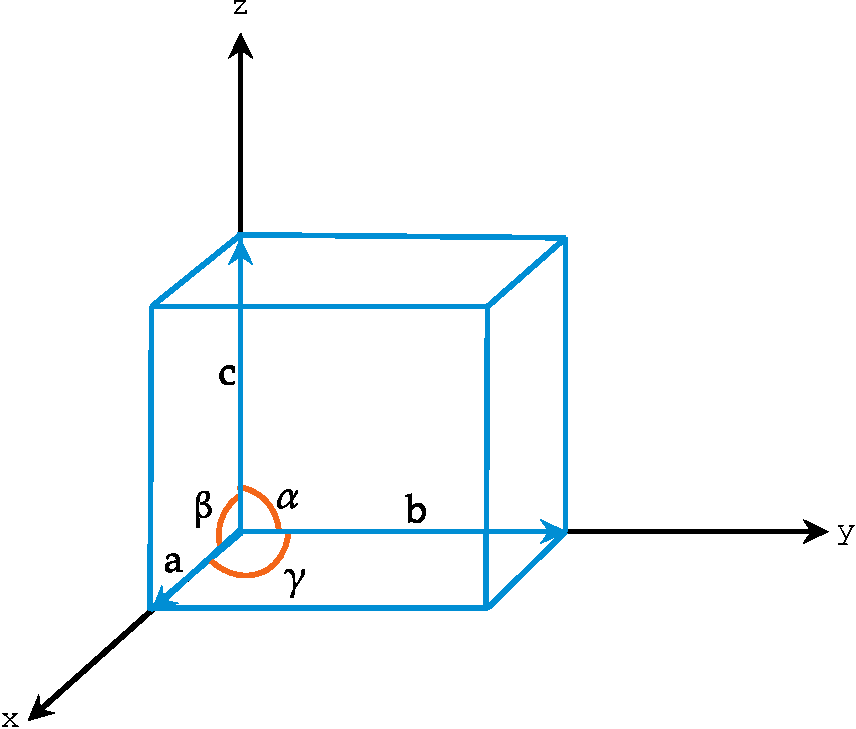
\includegraphics[height=6cm,width=6cm]{Unitcell}
		\caption{Unitcell}
		\label{}
	\end{figure}
If atoms are existing only at the corners of  the unit cell, the seven crystal systems will yield seven types of lattices.
\begin{table}[H]
	\begin{center}
	\renewcommand*{\arraystretch}{1.6}
		\arrayrulecolor{ocre}
	\begin{tabular}{|p{3.5cm}|p{3.5cm}|p{3.5cm}|}
		\hline \text { \textbf{System} } & \text { \textbf{Parameters} } & \text { \textbf{Interaxial Angles} } \\\hline
		\text { Triclinic } &$  \mathrm{a} \neq \mathrm{b} \neq \mathrm{c} $ & $ \alpha \neq \beta \neq \gamma $ \\\hline
		\text { Monoclinic } & $ \mathrm{a} \neq \mathrm{b} \neq \mathrm{c} $ & $ \alpha=\gamma=90^{\circ} \neq \beta  $\\\hline
		\text { Orthorhombic } & $ \mathrm{a} \neq \mathrm{b} \neq \mathrm{c} $ & $ \alpha=\beta=\gamma $ \\\hline
		\text { Tetragonal } & $ \mathrm{a}=\mathrm{b} \neq \mathrm{c} $ & $ \alpha=\beta=\gamma $ \\\hline
		\text { Cubic } & $ \mathrm{a}=\mathrm{b}=\mathrm{c} $ & $ \alpha=\beta=\gamma=90^{\circ} $ \\\hline
		\text { Hexagonal } & $ \mathrm{a}=\mathrm{b} \neq \mathrm{c} $ & $ \alpha=\beta=90^{\circ}, \gamma=120^{\circ} $ \\\hline
		\text { Rhombohedral } & $ \mathrm{a}=\mathrm{b}=\mathrm{c} $ & $ \alpha=\beta=\gamma \neq 90^{\circ} $ \\
		\hline
	\end{tabular}
\end{center}
\end{table}

\subsection{ Unit Cell and Primitive cell}
The unit cell is the smallest repetitive unit of a lattice. A primitive cell is the smallest possible unit cell of a lattice. The unit cell that contains one lattice point only at the corners is known as a primitive cell. 
\begin{note}
	\textbf{Difference between Unit Cell and Primitive Cell:}\\\\
	The unit cell differs from the primitive cell in that it is not restricted to being the equivalent of one lattice point. The primitive cell always contains lattice points only at corners.
\end{note}
\subsubsection{Non- primitive unit cell}
In a non-primitive unit cell lattice points are present not only at the corners but also at some specific position. They are,
\begin{enumerate}
	\item \textbf{BCC (Body Centred Cubic Unit Cell)}\\\\
	Lattice points at corners and body centre\\
	Total lattice point = 8 + 1= 9
	\item \textbf{FCC (Face Centred Cubic Unit Cell)}\\\\
	Lattice points at corners and at every faces\\
	Total lattice points = 8 + 6= 14
	\item \textbf{End Centred Unit Cell}\\
	Lattice points at all corners and at any two opposite faces\\\\
	Total lattuce point = 8 + 2= 10
	\item \textbf{Edge Centred Unit Cell (Hypothetical)}\\
	Lattice points at all corners and all edges\\
	Total lattice point = 8 + 12= 20
\end{enumerate}
	\subsection{Calculation of total number of lattice points per unit cell (z)}
	The number of lattice points tells you the number of atoms that are required to define your basis.
	\begin{equation*}
	z= \text{Total lattice point} \times \text{Contribution}
	\end{equation*}
\begin{enumerate}
		\item SCC
		\begin{align*}
		z&= \text{Contribution from all corners}\\
		&=8 \times \frac{1}{8}\\
		&=1
		\end{align*}
		\item BCC
		\begin{align*}
		z&= (\text{Corner} + \text{Body center})\\
		&= \left( 8 \times \frac{1}{8}\right)  + 1\\
		&= 2
		\end{align*}
		\item FCC
		\begin{align*}
		z&= (\text{Corner} + \text{Face center})\\
		&= \left( 8 \times \frac{1}{8}\right)  + 6 \times \frac{1}{2}\\
		&= 4
		\end{align*}
		\item End centred
		\begin{align*}
		z&= (\text{Corner} + \text{Any two opposite faces })\\
		&= \left( 8 \times \frac{1}{8}\right)  + 2 \times \frac{1}{2}\\
		&=2
		\end{align*}
		\item Edge centred
		\begin{align*}
		z&= \text{(Corners + edges) }\\
		&= \left( 8 \times \frac{1}{8}\right)  + \left( 12 \times \frac{1}{4}\right) \\
		&=4\\
		\end{align*}
	\end{enumerate}
\begin{table}[H]
	\renewcommand*{\arraystretch}{1.5}
	\begin{tabular}{|p{3 cm}|p{3 cm}|p{1 cm}|p{3.5cm}|p{5cm}| }
		\hline
		
		Crystal systems&\multicolumn{2}{|c|}{Bravais Lattices}& Unit cell parameters& Examples \\\hline 
		Cubic & Primitive \newline Body- centered \newline Face- centered &3& $a=b=c$ \newline $\alpha = \beta = \gamma = 90^{0}$ & NaCl, Zinc blende, Cu, Ag, Au, K, Na, Li \\ \hline 
		Tetragonal & Primitive \newline Body- centered & 2&$a=b \neq c$ \newline $\alpha = \beta = \gamma = 90^{0}$ & $SnO_{2}, TiO_{2}, CaSO_{4},$ \newline  $K_{4}[Fe(CN)_{6}].3H_{2}O$, Urea\\ \hline
		Hexagonal & Primitive &1& $a=b \neq c$ \newline $\alpha = \beta =  90^{0}$ \newline $\gamma = 120^{0}$ & Graphite, ZnO, CdS\\ \hline
		Rhombohedral & Primitive & 1&$a=b = c$ \newline $\alpha = \beta = \gamma \neq 90^{0}$& Calcite $(CaCO_{3})$, Cinnabar (HgS)\\ \hline
		Orthorhombic & Primitive \newline Body- centered \newline face- centered \newline End- centered &4& $a \neq b \neq c$ \newline $\alpha = \beta = \gamma = 90^{0}$& Rhombic sulphur, $KNO_{3}, BaSO_{4}$\\ \hline
		Monoclinic & Primitive   \newline End- centered &2& $a \neq b \neq c$ \newline $\alpha  = \gamma = 90^{0}$ \newline $ \beta \neq 90^{0} $ & {Monoclinic sulphur} $Na_{2}SO_{4}.10H_{2}O,$   $CaSO_{4}.2H_{2}O$ (Gypsum)\\ \hline
		Triclinic & Primitive&1 \multirow{1}{2cm}{14}& $a \neq b \neq c$ \newline $\alpha  \neq \beta \neq \gamma \neq 90^{0} $  & $K_{2}Cr_{2}O_{7}, CuSO_{4}.5H_{2}O, H_{3}BO_{3}$\\ \hline
	\end{tabular}
	\label{1}
	\caption{Crystal systems and Bravais lattices}
\end{table}

\section{Characterestics of the unit cell of a cubic system}
\begin{itemize}
	\item  Volume of a unit cell, $V=a \times b \times c$
	\item Mass and density of a unit cell:
	\begin{align*}
	\text{The mass of unit cell} &= \text{Number of atoms or molecules in the cell $\times$ Mass of each atom}\\
	\text{or,}\ m&=p \times m_{a}\quad \text{or}\quad  m=p \times \frac{M}{N_{a}} \\
	\text{Where,}\ M&= \text{molecular weight of the substance}\\
	\therefore \quad \text{Density,} d&=\frac{p \frac{M}{N_{a}}}{V}\\&=\frac{p M}{V N_{a}}
	\end{align*}
	If edge $\mathrm{a}$, is given in picometre then
	$$
	\mathrm{d}=\frac{\mathrm{pM}}{\mathrm{a}^{3} \mathrm{~N}_{\mathrm{a}} \times 10^{-30}} \mathrm{~g} / \mathrm{cm}^{3}
	$$
	\item Number of atoms (N) in a unit cell or the total number of atoms per unit cell is given by $$N=N_{i}+\frac{N_{f}}{2}+\frac{N_{c}}{8}$$ where $N_{i}=$ no. of body centred or interior atoms \\$N_{f}=$ no. of face centered atoms\\ $\mathrm{N}_{\mathrm{c}}=$ no. of corner atoms.
\end{itemize}

\section {Miller Indices}
In a crystal there exists \textbf{directions} and \textbf{planes} which contains a large concentration of atoms. For the analysis of crystal structure it is necssary to determine these planes and directions.
It is desirable to have a system of notation for planes such that the system specifies orientation without giving position in space, \textbf{Miller indices} are used for this purpose.
\begin{itemize}
	\item Miller indices for directions are simple as the representation of normal vectorial directions.
	\item Miller indices can be used equally well to describe lattices and crystals.
	\item The number of indices will match with the dimension of the lattice or the crystal . In 1-D there will be 1 index and for 2-D there will be 2 indices. etc.
\end{itemize}
\subsection{Miller Indices for Directions}
 A vector $\vec{r}$ passing from the origin to a lattice point can be written as
 \begin{equation}
 \vec{r}= p\vec{a}+q \vec{b}+r\vec{c}
 \end{equation}
  Where, $\vec{a}$, $\vec{b}$ ,$\vec{c}$ are basis vectors.\\
 \begin{minipage}{0.45\textwidth}
 \begin{figure}[H]
 	\centering
 	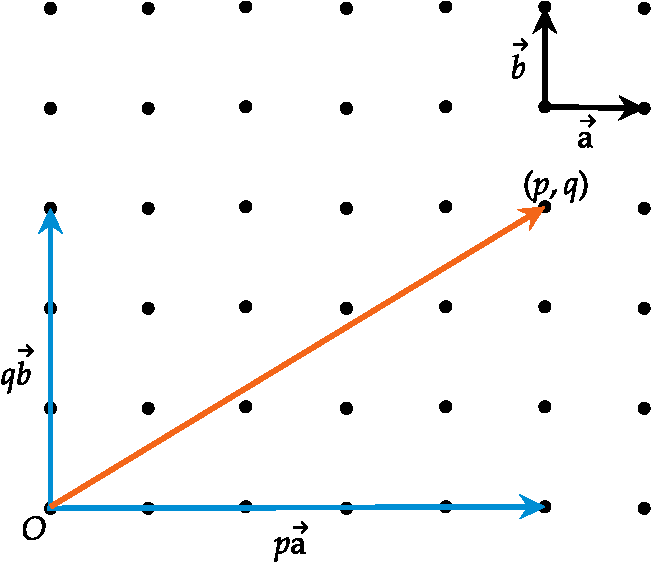
\includegraphics[height=5cm,width=5cm]{Miller indices- direction}
 	\caption{Miller indices In 2 Dimension}
 	\label{}
 \end{figure}
 \end{minipage}
\begin{minipage}{0.45\textwidth}
	\begin{figure}[H]
		\centering
		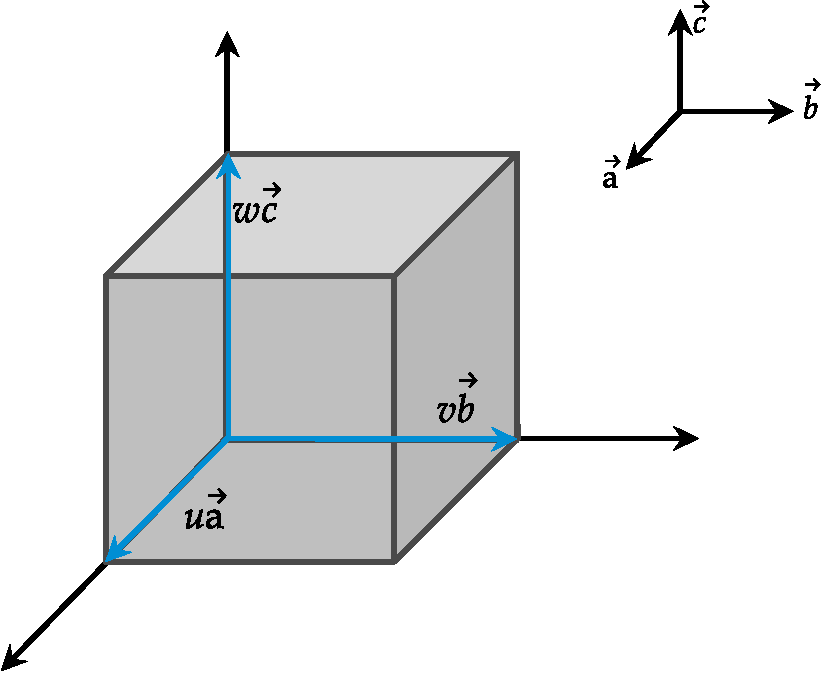
\includegraphics[height=5cm,width=6cm]{miller indices direction3D}
		\caption{Miller Indices in 3 Dimension}
		\label{}
	\end{figure}
\end{minipage}
 
 
  \subsubsection{Finding Miller Indices for Any Arbitrary Direction}
  \begin{enumerate}
  	\item Subtract the coordinates of the end points from the starting point(may be the origin) of the vector denoting the direction.
  	\item Enclose the coordinate in square bracket remove the comma and write the the negative number(if any) with a bar.
  	\item Factor out the common factor.
  	  \end{enumerate}
  	\begin{example}$\left. \right. $\\
  		\begin{minipage}{0.65\textwidth}
  			\begin{enumerate}
  				\item 	\begin{align*}
  			\text{Coordinates of the end point}&=(4,5)\\
  				\text{Coordinates of the starting point}&=(0,0) \text{(origin)}\\
  				\rightarrow &(4,5)
  				\end{align*}
  					\item 	\begin{align*}
  				\text{Miller indices}&=[4 \quad 5]\\
  			\end{align*}
  			\end{enumerate}
  		
  		
  		\end{minipage}\hfil
  	\begin{minipage}{0.25\textwidth}
  		\begin{figure}[H]
  			\centering
  			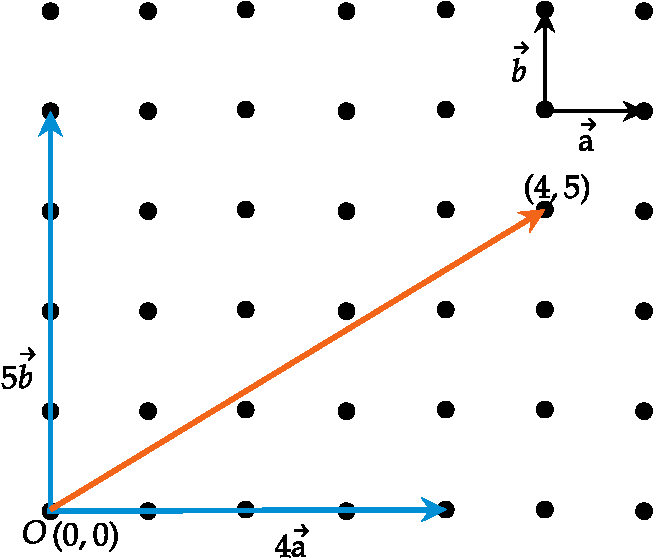
\includegraphics[height=4cm,width=4cm]{miller indices direction eg}
  			\caption{ Miller indices direction }
  			\label{}
  		\end{figure}
  	\end{minipage}
  		
  	\end{example}
\subsubsection{Family of direction}
These are the set of directions related by symmetry operations of the lattice or the crystal. Angle brackets $<$ indicate a family of directions. 
\begin{example}
	In a cubic system $\langle 100\rangle$ includes these directions $[100],[\overline{1} 00],[010],[0 \overline{1} 0],[001]$, and $[00 \overline{1}]$.
\end{example}
\begin{figure}[H]
	\centering
	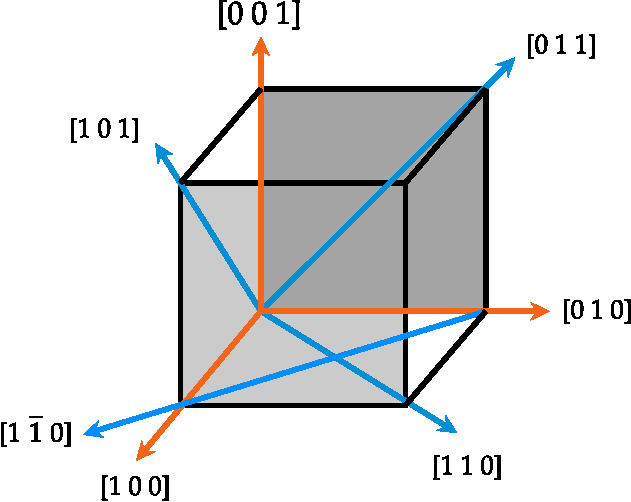
\includegraphics[height=4cm,width=5cm]{Miller indices- family of direction}
	\caption{Family of direction for $\langle 100\rangle$}
	\label{}
\end{figure}
\subsection{Miller Indices for Planes}
\begin{align*}
\text{For a plane with Weiss notation }	 &= \infty : 2b: c\\
\text{ A Reciprocal of coefficients} &=\frac{1}{\infty}, \frac{1}{2}, \frac{1}{1}\\
\text{ Multiplying by 2, to get whole numbers} &= 0, 2, 1\\
\text{Miller indices of the plane} &=0,1,2\\
i.e., h= 0, k&= 1, l= 2
\intertext{If Miller indices are \textbf{\textit{negative}} then these are represented by a bar,}
\text{i.e.,}(-h, -k, -l) &= (\bar{h}, \bar{k}, \bar{l})\\
 (-1, 2, 0) &= (\bar{1}, 2, 0)\\
(-2, -1, 3) &= (\bar{2}, \bar{1}, 3)
\end{align*}
\begin{exercise}
	Calculate the Miller Indices of crystal planes which cut through the crystal axes at \\
	(i) (2a, 3b, c)\\
	(ii) (a, b, c)\\
	(iii) (6a, 3b, 3c)\\
	(iv) (2a, -3b, -3c)
\end{exercise}	
\begin{answer}
	The Miller indices of given crystal planes can be calculated as follows;\\
	\vspace{0.6cm}
	\begin{minipage}{0.45\textwidth}
		(i) (2a, 3b, c)\\\\
		$\begin{array}{p{1cm} p{1cm} p{1cm} p{1.8cm}}
		a&b&c&\\
		2&3&1&intercepts\\
		1/2& 1/3&1& reciprocals\\
		3 & 2& 6& clear fractions
		\end{array}	$\\
		Hence, the Miller indices are \textbf{(3 2 6)}
	\end{minipage}
	\begin{minipage}{0.45\textwidth}
		(ii) (a, b, c)\\\\
		$\begin{array}{p{1cm} p{1cm} p{1cm} p{1.8cm}}
		a&b&c&\\
		1&1&1&intercepts\\
		1& 1&1& reciprocals\\
		1 & 1& 1& clear fractions
		\end{array}	$\\
		Hence, the Miller indices are \textbf{(1 1 1)}
	\end{minipage}	\\
	\begin{minipage}{0.45\textwidth}
		(iii) (6a, 3b, 3c)
		
		$\begin{array}{p{1cm} p{1cm} p{1cm} p{1.8cm}}
		a&b&c&\\
		6&3&3&intercepts\\
		1/6& 1/3&1/3& reciprocals\\
		1 & 2& 2& clear fractions
		\end{array}	$\\
		Hence, the Miller indices are \textbf{(1 2 2)}
	\end{minipage}
	\begin{minipage}{0.45\textwidth}
		(iv) (2a, -3b, -3c)
		
		$\begin{array}{p{1cm} p{1cm} p{1cm} p{1.8cm}}
		a&b&c&\\
		2&-3&-3&intercepts\\
		1/2& -1/3&-1/3& reciprocals\\
		3 & -2& -2& clear fractions
		\end{array}	$\\
		Hence, the Miller indices are $\mathbf{(3\  \bar{2}\ \bar{2})}$ 
	\end{minipage}		
\end{answer} 
\subsection{Properties of Miller Indices}
\begin{itemize}
	\item They represent the direction of the plane.
	\item Miller indices are always integers, never be fractional or infinite.
	\item Miller indices of a plane are proportional to the reciprocal of intercept of the plane on the three crystallographic axis x, y, z
	\item In Miller indices calculation, origin is never taken on the plane
	\item All parallel equidistant planes has the same miller indices.Thus miller indices define a set of parallel planes.
	\item A plane prallel to one of the coordinate axis has an intercepts of infinity.And miller indices equal to zero.
	\item If the miller indices of two planes have the same ratio ie(8,4,4),(4,2,2) or (2,1,1,) then the planes are parallel to each other.
	\item If (h,k,l) are miller indices of a plane , then the plane cut the axis in to h,k, and l equal segments respectively.
\end{itemize}
\begin{exercise}
	Find the Miller indices of the following shaded planes\\
	\begin{enumerate}
		\begin{minipage}{0.35 \textwidth}
			\item 	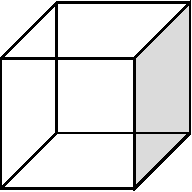
\includegraphics[width=0.3\textwidth]{mp1-crop}
		\end{minipage}	
		\begin{minipage}{0.35 \textwidth}
			\item 	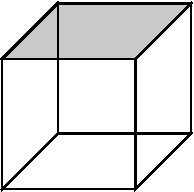
\includegraphics[width=0.3\textwidth]{mp2-crop}
		\end{minipage}
		\begin{minipage}{0.35 \textwidth}
			\item 	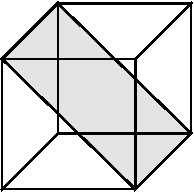
\includegraphics[width=0.3\textwidth]{mp3-crop}
		\end{minipage}
	\end{enumerate}
\end{exercise}
\begin{answer}
	Mark origin at a point one step away from the plane and calculate the Miller indices\\
	\begin{minipage}{0.45 \textwidth}
		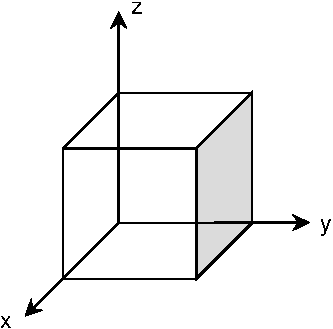
\includegraphics[width=0.5\textwidth]{mp1A-crop}
	\end{minipage}
	\begin{minipage}{0.45 \textwidth}
		$\begin{array}{p{1cm} p{1cm} |p{1cm}| p{1cm}}
		&x&y&z\\
		I &$\infty$ & 1&$\infty$\\
		R &0&1&0\\
		M&0&1&0
		\end{array}$
	\end{minipage}\\
	\begin{minipage}{0.45 \textwidth}
		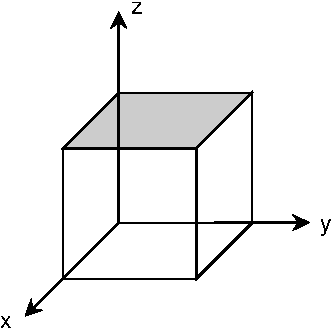
\includegraphics[width=0.5\textwidth]{mp2A-crop}
	\end{minipage}
	\begin{minipage}{0.45 \textwidth}
		$\begin{array}{p{1cm} p{1cm} |p{1cm}| p{1cm}}
		&x&y&z\\
		I &$\infty$ &$\infty$&1\\
		R &$\frac{1}{\infty}$&$\frac{1}{\infty}$&1\\
		M&0&0&1
		\end{array}$
	\end{minipage}\\
	\begin{minipage}{0.45 \textwidth}
		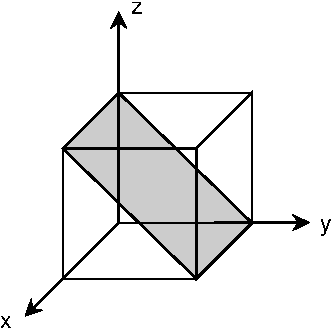
\includegraphics[width=0.5\textwidth]{mp3A-crop}
	\end{minipage}
	\begin{minipage}{0.45 \textwidth}
		$\begin{array}{p{1cm} p{1cm} |p{1cm}| p{1cm}}
		&x&y&z\\
		I &$\infty$ &1&1\\
		R &$\frac{1}{\infty}$&1&1\\
		M&0&1&1
		\end{array}$
	\end{minipage}\\
	\begin{minipage}{0.45 \textwidth}
		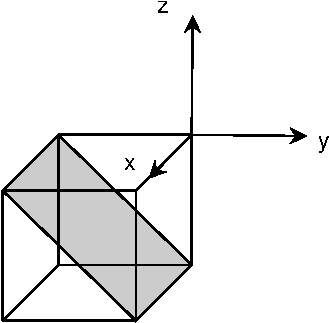
\includegraphics[width=0.5\textwidth]{mp3A1-crop}
	\end{minipage}
	\begin{minipage}{0.45 \textwidth}
		$\begin{array}{p{1cm} p{1cm} |p{1cm}| p{1cm}}
		&x&y&z\\
		I &$\infty$ &-1&-1\\
		R &$\frac{1}{\infty}$&-1&-1\\
		M&0&$\bar{1}$&$\bar{1}$
		\end{array}$
	\end{minipage}\\
Where I represents intercepts,R represents reciprocal of intercepts and M represents corresponding Miller indices.
	If all the Miller indices are multiplied by -1 the drawing of the plane doesn't change.
\end{answer}

\begin{note}
	Miller indices of a crystal plane that is \textbf{\textit{parallel}} to one of the axes is zero.\\
	Eg: $(1, 0, 0)$ corresponds to a plane parallel to y and z axes\\
	$(1, 1, 0)$ corresponds to a plane parallel to z- axis
\end{note}
\textbf{Examples For Some Miller Planes}

\begin{center}
	\begin{figure}[H]
		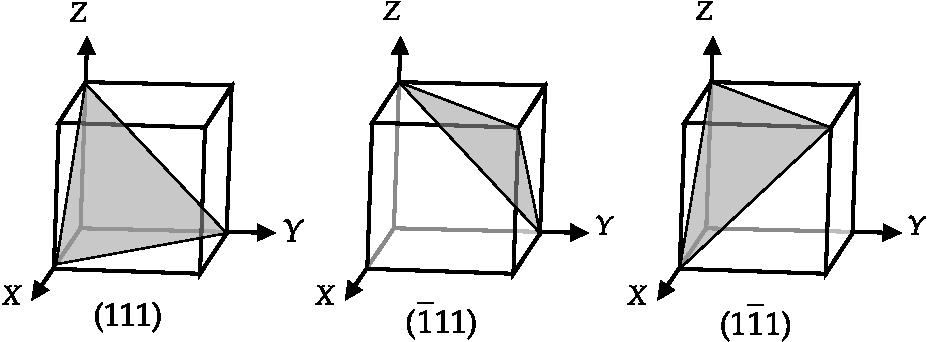
\includegraphics[width=0.5\textwidth]{plane1}\\
		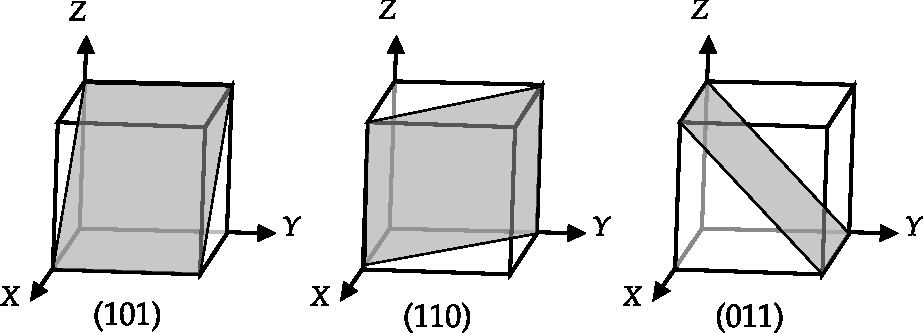
\includegraphics[width=0.5\textwidth]{plane2}\\
		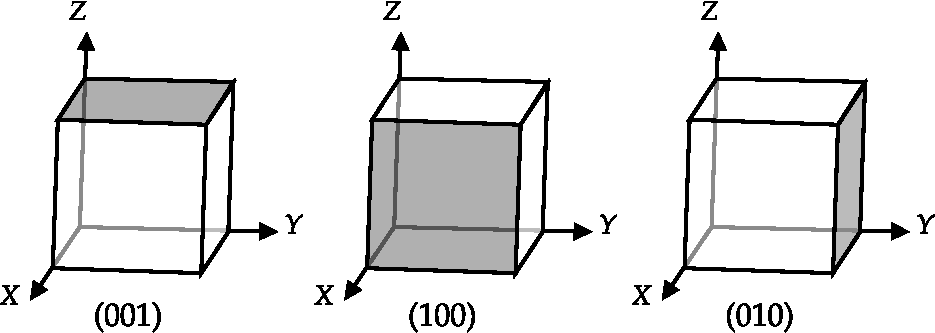
\includegraphics[width=0.5\textwidth]{plane3}
	\end{figure}
\end{center}

\newpage
\subsection {Interplanar Distance Ratio}
For the simple cubic lattice, the planes 100,110 and 111 completely describe the lattice structures.\\
Calculating the inter planar distances, we get\\
$\begin{aligned}
d_{100}= \frac{a}{\sqrt{1^{2}+0^{2}+0^{2}}}= a\\\\
d_{110}= \frac{a}{\sqrt{1^{2}+1^{2}+0^{2}}}= \frac{a}{\sqrt{2}}\\\\
d_{111}= \frac{a}{\sqrt{1^{2}+1^{2}+1^{2}}}= \frac{a}{\sqrt{3}}\\
\text {Interplanar distance ratio,}\\
d_{100}: d_{110}: d_{111} &= a: \frac{a}{\sqrt{2}}: \frac{a}{\sqrt{3}}\\
&= 1: \frac{1}{\sqrt{2}}: \frac{1}{\sqrt{3}}\\
&= 1: 0.707: 0.577\\
\end{aligned}$\\
Similarly we can find out the interplanar distance ratio of BCC and FCC.
\begin{eBox}
	$\begin{aligned}
	\textbf{SC} &\longrightarrow \ d_{100}: d_{110}: d_{111} &= 1: \frac{1}{\sqrt{2}}: \frac{1}{\sqrt{3}} &= 1: 0.707: 0.577\\
	\textbf{BCC} &\longrightarrow \ d_{200}: d_{110}: d_{222} &= \frac{1}{2}: \frac{1}{\sqrt{2}}: \frac{1}{2 \sqrt{3}} &= 1: 1.414: 0.577\\
	\textbf{FCC} &\longrightarrow \ d_{200}: d_{220}: d_{111} &= \frac{1}{2}: \frac{1}{2 \sqrt{2}}: \frac{1}{\sqrt{3}} &= 1: 0.707: 1.154
	\end{aligned}$
\end{eBox}
\subsection{Angle Between Planes}
Consider two planes having Miller indices $(h_{1} k_{1} l_{1})$ and $(h_{2} k_{2} l_{2})$. The angle between these two planes can be calculated by using the formula,

\begin{center}
	\framebox{
		\parbox[t][1.5cm]{6cm}{
			
			\addvspace{0.2cm} \centering 
			
			$\begin{aligned}
			cos \theta &= \frac{h_{1}h_{2}+k_{1}k_{2}+l_{1}l_{2}}{\sqrt{h_{1}^{2}+k_{1}^{2}+l_{1}^{2}}\sqrt{h_{2}^{2}+k_{2}^{2}+l_{2}^{2}}}
			\end{aligned}$} }
\end{center}

\begin{exercise}
	Find the angle between the planes (1 1 0) and (1 1 1)
\end{exercise}
\begin{answer}
	\begin{align*}
	cos \theta &= \frac{h_{1}h_{2}+k_{1}k_{2}+l_{1}l_{2}}{\sqrt{h_{1}^{2}+k_{1}^{2}+l_{1}^{2}}\sqrt{h_{2}^{2}+k_{2}^{2}+l_{2}^{2}}}\\
	cos \theta &=\frac{1\times 1+ 1\times 1 +0 \times 1}{\sqrt{1^{2}+1^{2}+0^{2}}\sqrt{1^{2}+1^{2}+1^{2}}}\\
	&=\frac{2}{\sqrt{2}\sqrt{3}}\\
	&=\frac{\sqrt{2}\sqrt{2}}{\sqrt{2}\sqrt{3}}= \frac{\sqrt{2}}{\sqrt{3}}\\
	\theta &= cos^{-1} \left( \frac{\sqrt{2}}{\sqrt{3}}\right) \\
	\theta &= 35.3^{0}
	\end{align*}
\end{answer}
\section{Distribution of atoms in the atomic planes of a simple cubic crystal}
	Let $a$ be the lattice constant in millimetre and $r$ be the radius of the atom in millimetre.
\begin{enumerate}
	\item (010) Plane \\
	\begin{align*}
	\text{Area of the plane is} &= a^{2}\\
	\text{Atoms per sq $\mathrm{mm}$ }&=\frac{1}{a^{2}}=\frac{1}{4 r^{2}}
	\end{align*}

	\item (110) Plane
		\begin{align*}
	\text{Area of the plane is} &=\sqrt{2} a^{2}\\
	\text{Atoms per sq $\mathrm{mm}$ }&=\frac{1}{\sqrt{2} a^{2}}\\&=\left[\frac{1}{\sqrt{2}}\right]\left[\frac{1}{4 r^{2}}\right]
	\end{align*}

	\item  (111) Plane
	\begin{align*}
	\text{Area of the plane is} &=\frac{\sqrt{3}}{2} a^{2}\\
	 \text{Number of atoms} &=\frac{1}{6} \times 3=\frac{1}{2}\\
	\text{Atoms per sq $\mathrm{mm}$ }&=\frac{1 / 2}{\frac{\sqrt{3}}{2} a^{2}}=\frac{1}{\sqrt{3} a^{2}}\\&=\left(\frac{1}{\sqrt{3}}\right)\left[\frac{1}{4 r^{2}}\right]
\end{align*}

\end{enumerate}

\section{Symmetry in Crystals}
\begin{enumerate}
	\item \textbf{Plane of symmetry}\\
	An imaginary plane which can divide the crystal into two equal halves such that one is the mirror image of the other.\\
	A cubic crystal, for example, has two types of plane of symmetry.
	\begin{enumerate}[label=\alph*., itemsep=\baselineskip]
		\item Rectangular planes of symmetry\\
		The planes are situated at the center and parallel to the opposite faces.\\
		Since a cubic crystals have six faces, it has \textbf{\textit{three}} rectangular plane of symmetry.\\
		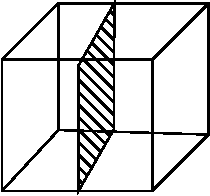
\includegraphics[width=0.15\textwidth]{p1-crop}
		\item Diagonal plane of symmetry\\
		The planes are passing through opposite edges.\\
		As they lie on the diagonal of opposite faces, these are known as diagonal planes of symmetry.\\
		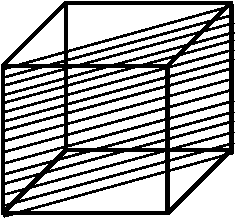
\includegraphics[width=0.15\textwidth]{p2-crop}	\\\\
		In a cubic crystal there are 3 rectangular planes of symmetry and 6 diagonal planes of symmetry. 		
	\end{enumerate}
	
	\begin{figure}[h]
		\begin{minipage}{0.3\textwidth}	
			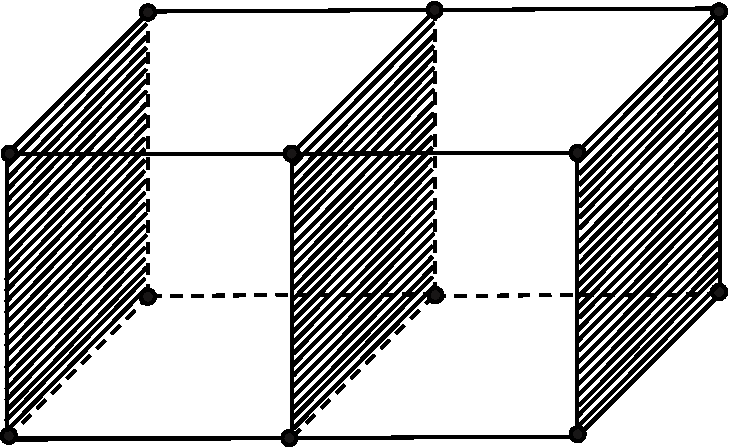
\includegraphics[width=0.75\textwidth]{P C(100)-crop}
			\caption*{\raggedright{ (100)}}
		\end{minipage}
		\begin{minipage}{0.3\textwidth}
			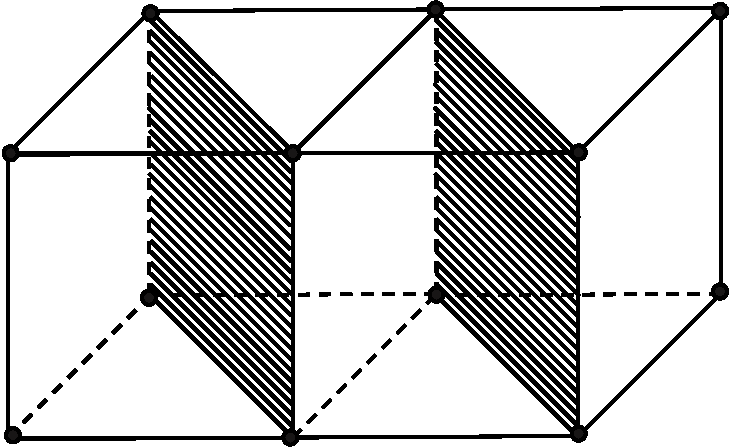
\includegraphics[width=0.75\textwidth]{P C(110)-crop}
			\caption*{\raggedright{ (110)}}
		\end{minipage}
		\begin{minipage}{0.3\textwidth}
			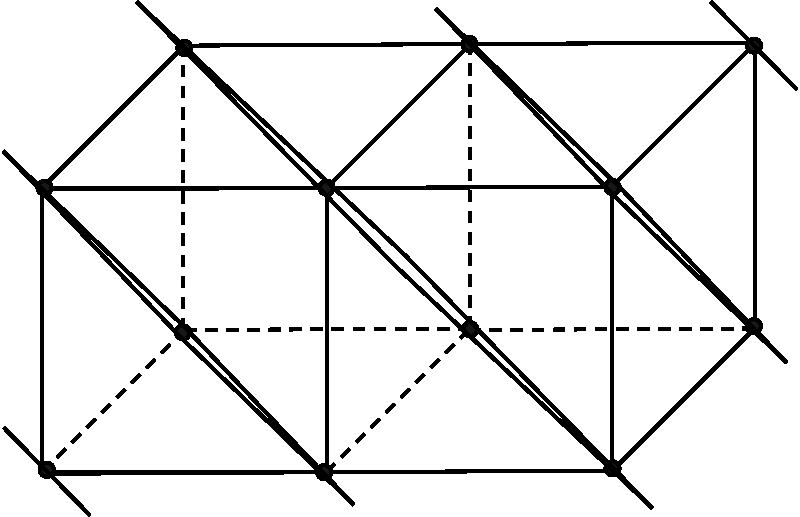
\includegraphics[width=0.75\textwidth]{P C(111)-crop}
			\caption*{\raggedright{ (111)}}
		\end{minipage}
	\end{figure}
	\begin{figure}[h]
		\begin{minipage}{0.3 \textwidth}
			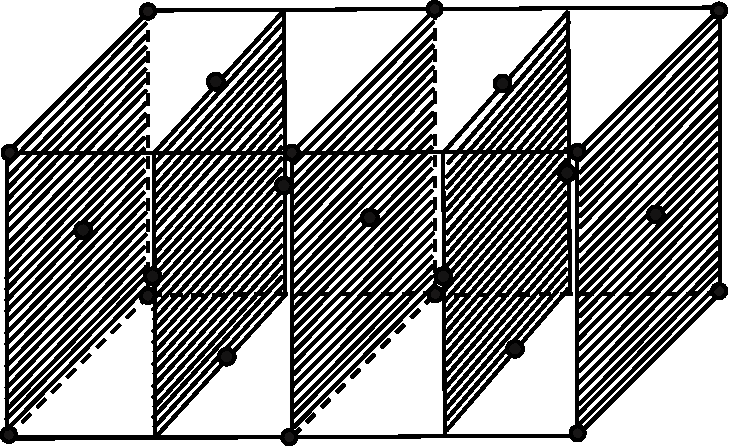
\includegraphics[width=0.75\textwidth]{P C(200)-crop}
			\caption*{\raggedright{ (200)}}
		\end{minipage}
		\begin{minipage}{0.3 \textwidth}
			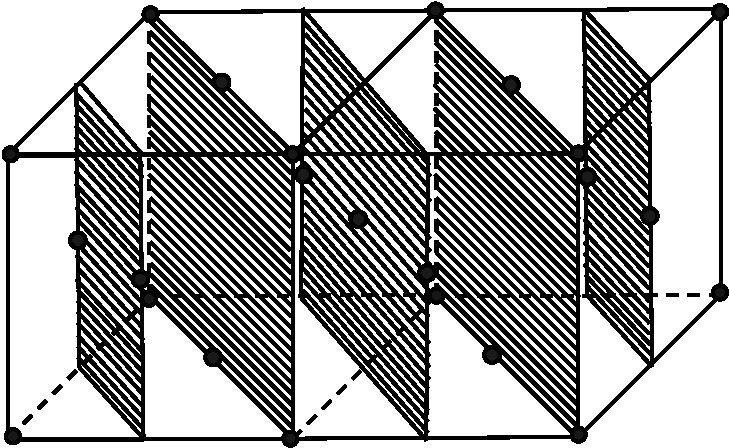
\includegraphics[width=0.75\textwidth]{P C(220)-crop}
			\caption*{\raggedright{ (220)}}
		\end{minipage}
		\begin{minipage}{0.3 \textwidth}
			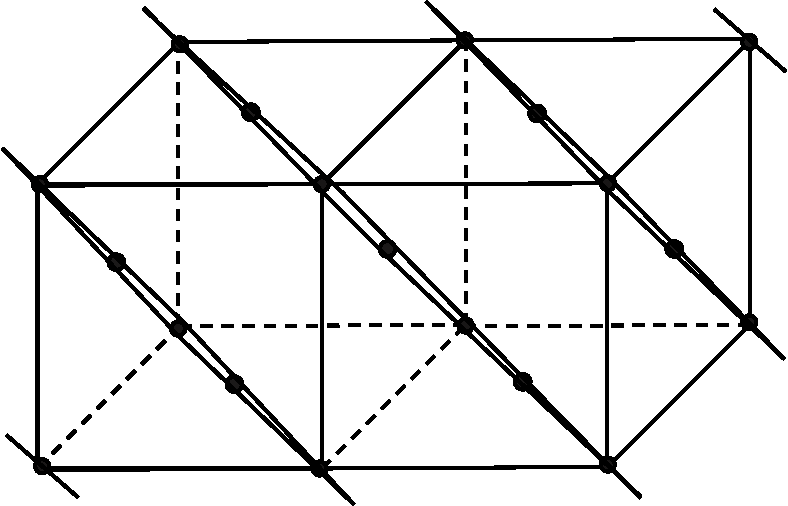
\includegraphics[width=0.75\textwidth]{P C(111-2)-crop}
			\caption*{\raggedright{ (111)}}
		\end{minipage}
	\end{figure}
	\begin{figure}[h]
		\begin{minipage}{0.3 \textwidth}
			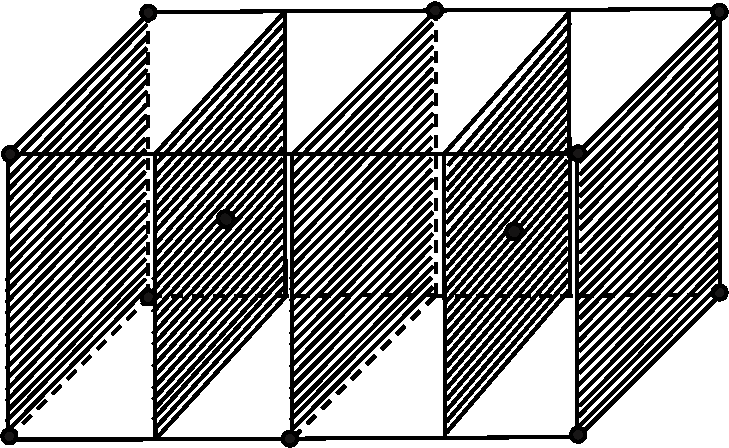
\includegraphics[width=0.75\textwidth]{P C(200-3)-crop}
			\caption*{\raggedright{ (200)}}
		\end{minipage}
		\begin{minipage}{0.3 \textwidth}
			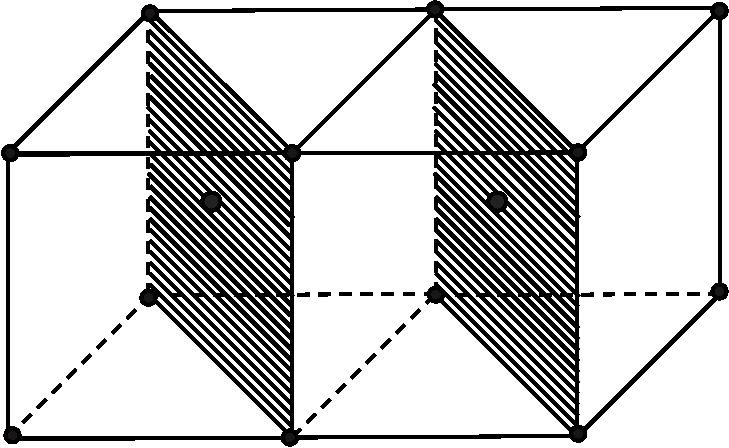
\includegraphics[width=0.75\textwidth]{P C(110-3)-crop}
			\caption*{\raggedright{ (110)}}
		\end{minipage}
		\begin{minipage}{0.3 \textwidth}
			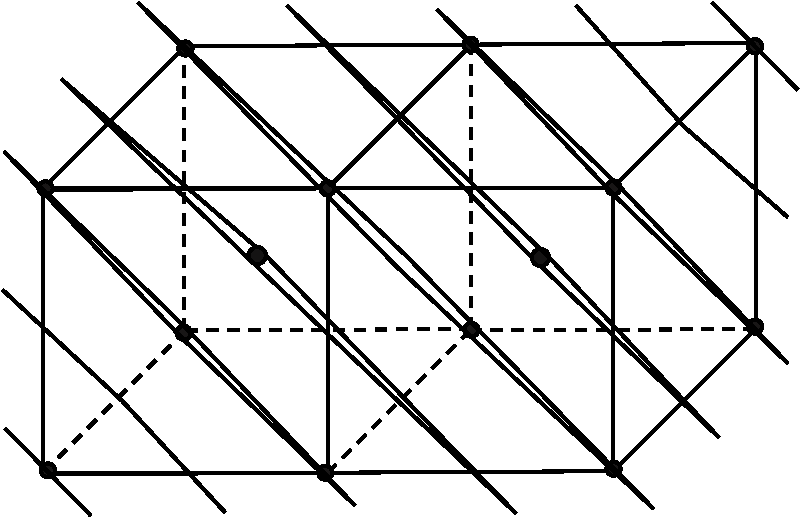
\includegraphics[width=0.75\textwidth]{P C(222)-crop}
			\caption*{\raggedright{ (222)}}
		\end{minipage}
		\caption{Lattice Planes in a Cubic System}
	\end{figure}

	\item \textbf{Axis or line of symmetry}\\
	An imaginary line (or axis) about which the crystal may be rotated so that it presents the same appearence more than once in a complete rotation through $360^{0}$.\\
	In a cubic crystal the axis of symmetry may be of three types depending upon the number of times the identical appearence occurs during the course of rotation.
	\begin{enumerate}[label=\alph*., itemsep=\baselineskip]
		\item Axis of two- fold symmetry (Diad axis)\\
		$\bullet$	The identical appearence of the cube occurs two times.\\
		$\bullet$	Original appearence is repeated as a result of rotation through $180^{0}$\\
		$\bullet$	For a cubic crystal, there are 6 diad axes.
		\item Axis of three- fold symmetry (Triad axis)\\
		$\bullet$ The identical appearence of the cube occurs three times.\\
		$\bullet$ Original appearence is repeated as a result of rotation through $120^{0}$\\
		$\bullet$ For a cubic crystal, there are 4 triad axes.
		\item Axis of four- fold symmetry (Tetrad axis)\\
		$\bullet$ The identical appearence of the cube occurs four times.\\
		$\bullet$ Original appearence is repeated as a result of rotation through $90^{0}$\\
		$\bullet$ For a cubic crystal, there are 3 tetrad axes.	
		\item Axis of six- fold symmetry (Hexad axis)\\
		$\bullet$ The identical appearence of the cube occurs six times.\\
		$\bullet$ Original appearence is repeated as a result of rotation through $60^{0}$\\
		$\bullet$ This axis of symmetry is possible in hexagonal crystals and not in cubic crystals.
		\begin{figure}[h]	
			\begin{minipage}{0.24\textwidth} 
				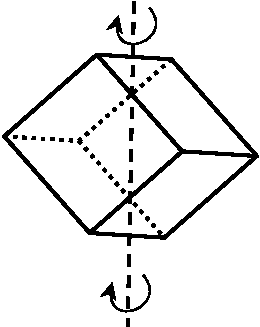
\includegraphics[width=0.8\textwidth]{c2-crop}
				\caption*{Two- fold axis}
			\end{minipage}
			\begin{minipage}{0.24\textwidth}\hfill
				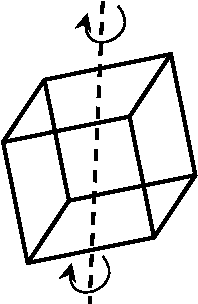
\includegraphics[width=0.45\textwidth]{c3-crop}
				\caption*{Three- fold axis}
			\end{minipage}
			\begin{minipage}{0.24\textwidth}\hfill
				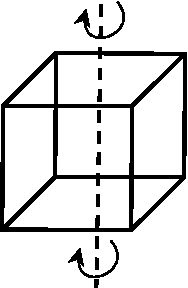
\includegraphics[width=0.45\textwidth]{c4-crop}
				\caption*{Four- fold axis}
			\end{minipage}
			\begin{minipage}{0.24\textwidth}\hfill
				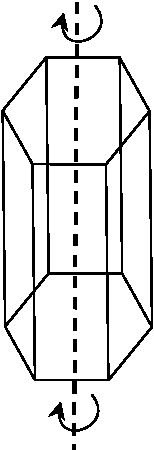
\includegraphics[width=0.45\textwidth]{c6-crop}
				\caption*{Six- fold axis}
			\end{minipage}
		\end{figure}
	\end{enumerate}
	\item \textbf{Center of symmetry}\\
	A point in the crystal that any line drawing through it intersects the surface of the crystal at equal distances on either side.\\
	A crystal may have one or more planes or axes of symmetry but it never has more than one center of symmetry which lies at the center of the cube.\\
	\begin{figure}[h]
		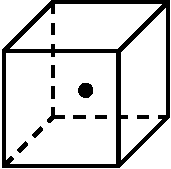
\includegraphics[width=0.15\textwidth]{centrsym-crop}
		\caption*{\raggedright{Centre of symmetry}}
	\end{figure}
\end{enumerate}
\begin{dBox}
	For a cubic crystal,\\
	$\begin{aligned}
	\text{Plane of symmetry}&= 3+6=9\\
	\text{Axes of symmetry}&= 3+4+6 =13\\
	\text{Centre of symmetry}&= 1\\
	\text{Total number of elements of symmetry}&= 9+13+1=23
	\end{aligned}$
\end{dBox}
\section {CLOSE PACKED STRUCTURES}
\subsection{Close packing in two dimensions}
$\left. \right. $
\subsubsection{Square close packing}
Each sphere is in contact with four of its neighbours. \\
Coordination number =4
\begin{figure}[H]
	\centering
	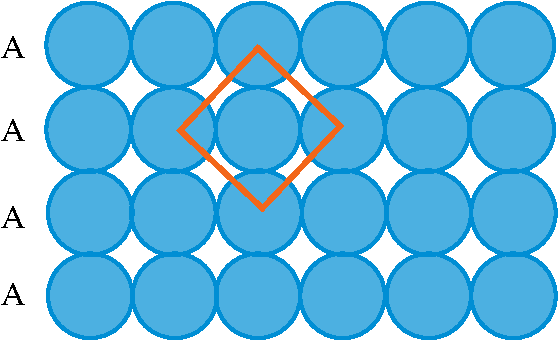
\includegraphics[width=0.40\textwidth]{2DCP-crop}
	\caption{Square close packing in 2- dimension}
	\label{}
\end{figure}

\subsubsection{Hexagonal close packing }
Each sphere is in contact with six of its neighbours.\\
Coordination number =6
\begin{figure}[H]
	\centering
	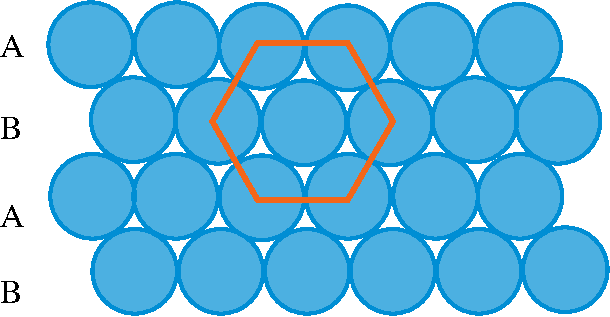
\includegraphics[width=0.45\textwidth]{2DCP1-crop}
	\caption{Hexagonal close packing in 2- dimension}
	\label{}
\end{figure}

\section{Close packing in three dimensions}
a)	From two dimensional square close packing\\
$\bullet$ AAA type arrangement\\
$\bullet$	The lattice generated is simple cubic lattice, and its unit cell is primitive cubic unit cell\\
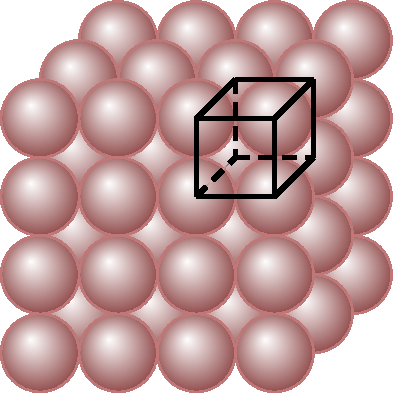
\includegraphics[width=0.35\textwidth]{ss1-crop}\\
b)	From two dimensional hexagonal close packing \\
\textit{(i) Covering tetrahedral voids.}\\
\begin{minipage}{0.45\textwidth}
	$\bullet$	ABAB type arrangement\\
	$\bullet$ Coordination number = 12\\
	$\bullet$ Crystal structure - hcp\\
	Eg: Mg, Zn
\end{minipage}
\begin{minipage}{0.45\textwidth}
	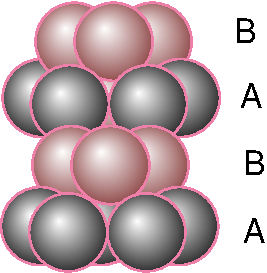
\includegraphics[width=0.35\textwidth]{ss2-crop}	
\end{minipage}
\newline
\textit{(ii) Covering octahedral voids}\\
\begin{minipage}{0.45\textwidth}
	$\bullet$ ABCABC type arrangement\\
	$\bullet$ Coordination number = 12\\
	$\bullet$ Crystal structure- ccp or fcc\\
	Eg: Cu, Ag
\end{minipage}
\begin{minipage}{0.45\textwidth}
	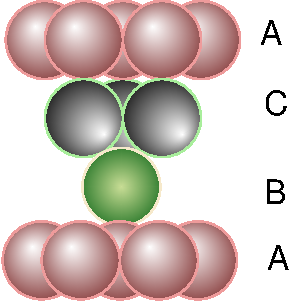
\includegraphics[width=0.35\textwidth]{ss3-crop}	
\end{minipage}\\
\begin{note}
	In addition to the above two types of arrangements, a third type of arrangement found in metals is body – centered cubic (bcc) structure. 
\end{note}
Eg: Alkali metals crystallize in bcc structure. Co-ordination number = 8\\
\begin{exercise}
	In a close packed structure of mixture oxides, the lattice is composed of oxide ions, one eighth of tetrahedral voids are occupied by divalent cations while one half of octahedral voids are occupied by trivalent cations. What is the formula of the oxide?
\end{exercise}
\begin{answer}
	$$\begin{aligned}
	\text{Number of oxide ions (O) per unit cell}&= 1\\
	\text{Number of tetrahedral voids per ion in lattice}&= 2\\
	\therefore \text{Number of divalent cation (A)} &= \frac{1}{8} \times 2 = \frac{1}{4}\\
	\text{Number of octahedral voids per ion in lattice}&= 1\\
	\therefore \text{Number of trivalent cations (B)}&= 1 \times \frac{1}{2} = \frac{1}{2}\\
	\text{Formula} &=A_{1/4}B_{1/2}O\\ &= AB_{2}O_{4}
	\end{aligned}$$
\end{answer}
\begin{exercise}
	Metallic gold crystallizes in the face- centered cubic lattice. The length of the cubic unit cell, $a = 4.070 A^{0}$. Calculate the closest distance between gold atoms and the density of gold. Atomic mass of Au = 197 amu
\end{exercise}
\begin{answer}
	In face- centered cubic cell,\\
	\begin{align*}
	\text{radius} &= \frac{\sqrt{2}a}{4}\\
	\therefore \text{closest distance between two atoms, diameter} &= 2 \times \frac{\sqrt{2}a}{4} = \frac{a}{\sqrt{2}}\\
	&= \frac{4.070}{\sqrt{2}} A^{0} = 2.878 A^{0}\\
	\text{Number of atoms in a face- centered unit cell} &= 8\left( \frac{1}{8}\right) + 6\left( \frac{1}{2}\right)\\
	\text{Mass of 4 atoms per unit cell} &= 4 \times 197 amu\\
	&= 4 \times 197 \times \left( 1.66 \times 10^{-24}\right) g\\
	&= 1.308 \times 10^{-21}g\\
	\text{volume of the unit cell}&= a^{3}= \left( 4.07 \times 10^{-8}\right) ^{3}cc\\
	\therefore \text{density of gold}&= \frac{1.308 \times 10^{-21}}{\left( 4.07 \times 10^{-8}\right) ^{3}} = 19.40 g/cc
	\end{align*}
\end{answer}
\subsection{Packing Fraction or Packing Efficiency}
Atomic packing factor (APF), packing efficiency, or packing fraction is the fraction of volume in a crystal structure that is occupied by constituent particles.\\ It is a dimensionless quantity and always less than unity.
\begin{enumerate}
	\item Simple Cubic Lattice\\
	Each unit cell effectively contains \textbf{\textit{one}} sphere\\
	\begin{align*}
	\text{The radius of the sphere, r}  &= \frac{a}{2}\\
	\therefore \text{Volume of the sphere} &= \frac{4}{3} \pi r^{3}\\
	&= \frac{4}{3} \pi \left( \frac{a}{2}\right) ^{3}\\
	\text{	Volume of the cube} &= a^{3}\\
	\therefore \text{Packing fraction} & = \frac{\frac{4}{3} \pi \left( \frac{a}{2}\right) ^{3}}{a^{3}}\\
	&= \frac{\pi}{6} = 0.524\\
	\therefore		\text{Packing efficiency} &= 52.4 \%
	\end{align*}
	\begin{minipage}{0.45 \textwidth}\hfill
		\begin{figure}[H]
			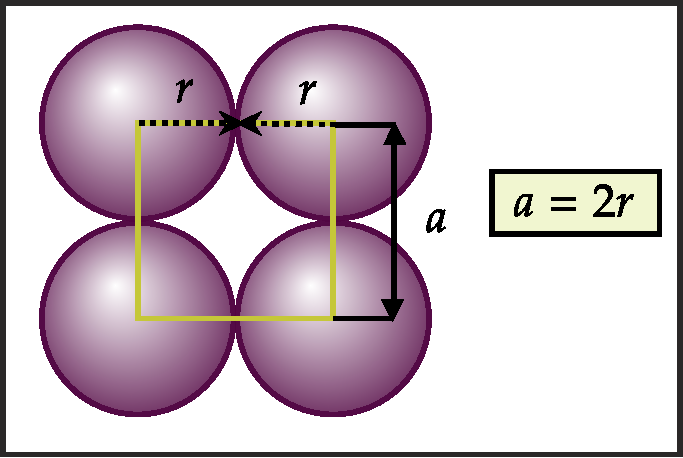
\includegraphics[width=0.8\textwidth]{sc.PNG-crop}
		\end{figure}
	\end{minipage}
	\begin{minipage}{0.45 \textwidth}\hfill
		\begin{figure}[H]
			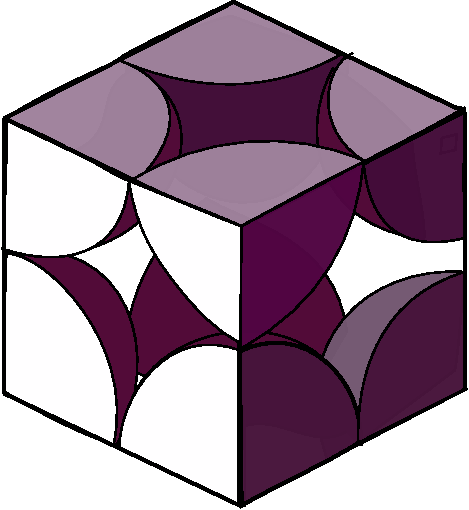
\includegraphics[width=0.45\textwidth]{sc1}
		\end{figure}
	\end{minipage}
	\item Body- Centerd Cubic Lattice (BCC)\\
	Each unit cell effectively contains \textbf{\textit{two}} spheres.\\
	$\begin{aligned}
	\text{The radius of the sphere, r} &= \frac{\sqrt{3}}{4}a\\
	\text{The volume of two spheres} &= 2 \times \frac{4}{3} \pi \left( \frac{\sqrt{3}}{4}a\right) ^{3}\\
	\text{Packing fraction} &= \frac{\sqrt{3} \pi}{8} = 0.6802\\
	\therefore \text{Packing efficiency} &= 68.02 \%
	\end{aligned}$\\
	\begin{minipage}{0.45 \textwidth} \hfill
		\begin{figure}[H]
			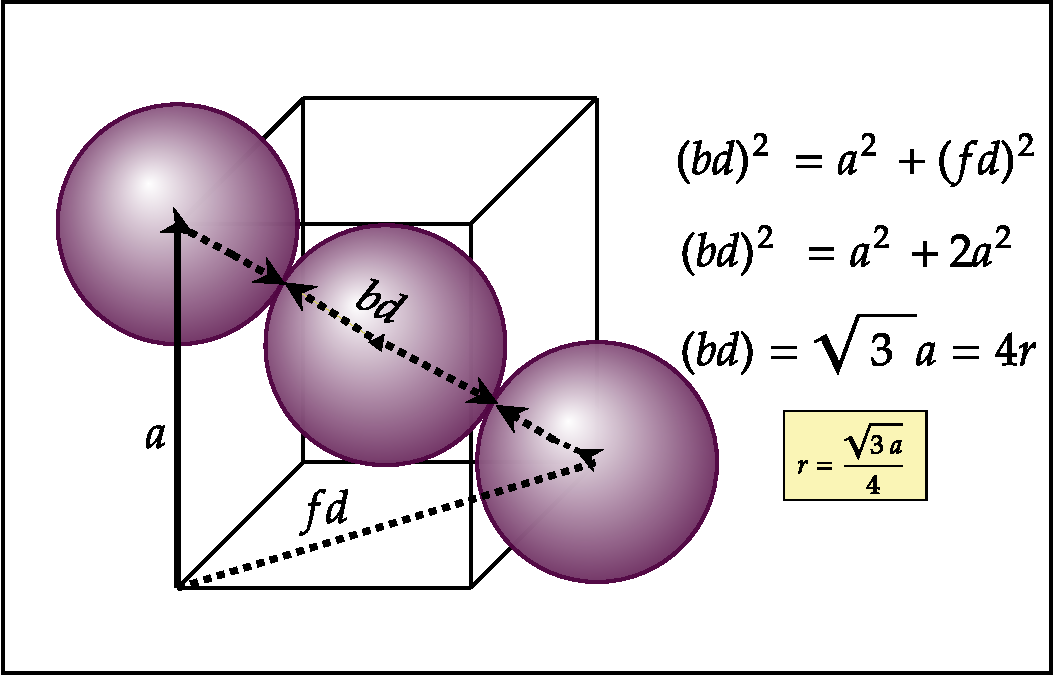
\includegraphics[width=0.95\textwidth]{bcc-crop}
		\end{figure}
	\end{minipage}
	\begin{minipage}{0.45 \textwidth} \hfill
		\begin{figure}[H]
			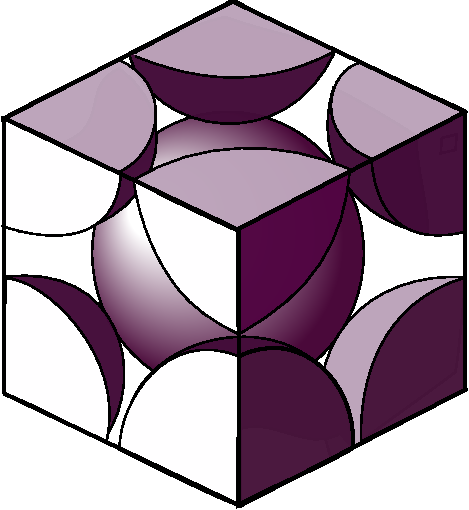
\includegraphics[width=0.6\textwidth]{bcc1}
		\end{figure}
	\end{minipage}\\
	\item Face- Centered Cubic (FCC) or Cubic Close Packing (CCP)\\
	Each unit cell effectively contains \textbf{\textit{four}} spheres
	$\begin{aligned}
	\text{The radius of the sphere, r} &= \frac{\sqrt{2}}{4}a\\
	\text{The volume of 4 spheres} &= 4 \times \frac{4}{3}	\pi \left( \frac{\sqrt{2}}{4}a\right) ^{3}\\
	\text{Packing fraction}&= \frac{\sqrt{2}}{6} \pi = 0.7404\\
	\therefore \text{Packing efficiency} &= 74.04 \%
	\end{aligned}$\\
	\begin{minipage}{0.45 \textwidth} \hfill
		\begin{figure}[H]	
			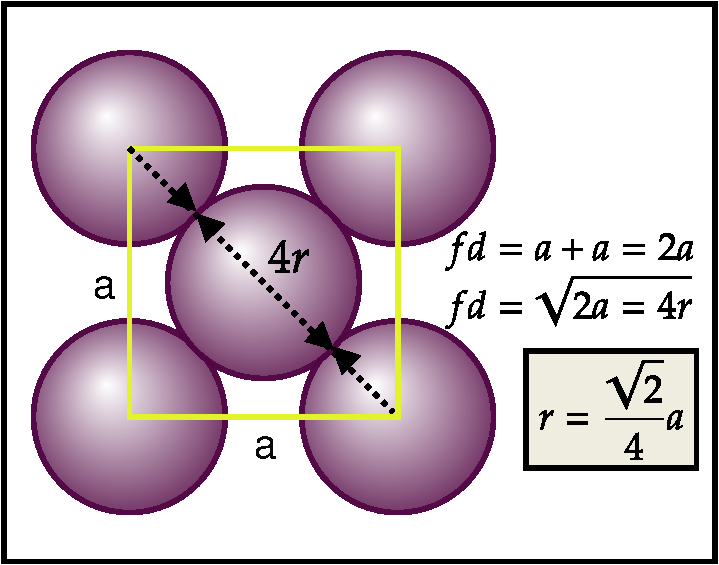
\includegraphics[width=0.75\textwidth]{fcc.PNG-crop}
		\end{figure}
	\end{minipage}
	\begin{minipage}{0.45 \textwidth} \hfill
		\begin{figure}[H]
			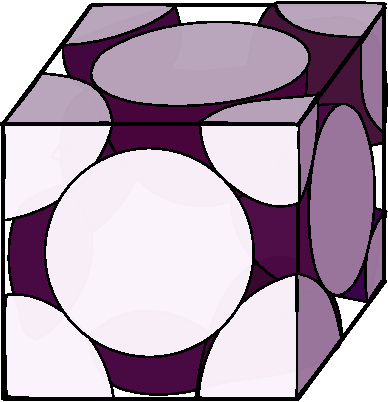
\includegraphics[width=0.35\textwidth]{fcc1}
		\end{figure}
	\end{minipage}
\end{enumerate}
Of the three cases discussed above, the \textbf{\textit{packing fraction is the largest in the case of fcc}} i.e, packing is the tightest.\\

\begin{note}
	$\begin{array}{p{3cm} p{3cm} p{3cm} }
	\text	{\textbf{Lattice type}} & \text{\textbf{Packing efficiency}}& \text{\textbf{Coordination number}}\\
	\text{Simple cubic}& 52.4 \% &6\\
	\text{BCC}& 68.02 \% & 8\\
	\text{FCC}& 74.04 \% & 12
	\end{array}	$\\
\end{note}
\begin{exercise}
	Calculate the packing efficiency and density of NaCl from the following data:\\
	$\begin{aligned}
	\text{Radius of sodium ion} &= 0.98 A^{0}\\
	\text{Radius of chloride ion} &= 1.81 A^{0}\\
	\text{Atomic mass of sodium}&= 22.99 amu\\
	\text{Atomic mass of chlorine} &= 35.45 amu
	\end{aligned}$
\end{exercise}
\begin{answer}
	The $Na^{+}$ and $Cl^{-}$ ions touch along the cube edges.\\
	$\begin{aligned}
	\text{Lattice parameters, a} &= 2\left( r_{Na^{+}}+ r_{Cl^{-}} \right) = 5.58 A^{0}\\
	\text{Packing fraction}&= \frac{\text{Volume of ions present in the unit cell}}{\text{Volume of the unit cell}}\\
	&= \frac{4(4/3)\pi r_{Na^{+}}^{3}+ 4(4/3)\pi r_{Cl^{-}}^{3}}{a^{3}}\\
	&=66.3 \%\\
	\text{Density}&= \frac{\text{Mass of the unit cell}}{\text{Volume of the unit cell}}\\
	&= \frac{4(22.99+ 35.45) \times 1.66 \times 10^{-27}}{(5.58 \times 10^{-10})^{3}} kgm^{-3}\\
	&=2.23 gcm^{-3}
	\end{aligned}$
\end{answer}
\begin{exercise}
	A flat surface is covered with non- overlapping disks of same size. What is the largest fraction of the area that can be covered?
\end{exercise}
\begin{answer}
	Let the radius of the circular disk is \textit{a}.\\
	\begin{align*}
	\text{Then, area of the circular disk}&= \pi r^{2}\\
	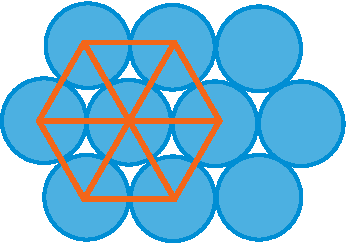
\includegraphics[width=0.30\textwidth]{q1-crop}\\
	\intertext{Here, Centers of three disks makes an equilateral triangle with area}\text{Area}&= \frac{\sqrt{3}a^{2}}{4} = \frac{\sqrt{3}(2r)^{2}}{4}\\
	\therefore \text{Packing fraction of the triangular lattice}&= \left( \frac{\frac{3}{6} \times \pi r^{2}}{\frac{\sqrt{3}a^{2}}{4}}\right) \\
	&= \left( \frac{\frac{3}{6} \pi r^{2}}{\frac{\sqrt{3}\times (2r)^{2}}{4}}\right) \\
	&=\frac{\pi}{2 \sqrt{3}}\\
	 \intertext{The fractional area of the flat surface that can be covered by these circular discs,}&=\frac{\pi}{2 \sqrt{3}}
	\end{align*}
\end{answer}
\colorlet{ocre1}{ocre!70!}
\colorlet{ocrel}{ocre!30!}
\setlength\arrayrulewidth{1pt}
\begin{table}[H]
	\centering
	\arrayrulecolor{ocre}
	\renewcommand{\arraystretch}{1.5}
	\begin{tabular}{|l|l|l|l|l|l|}
		\hline & $\mathrm{SC}$ & $\mathrm{BCC}$ & $\mathrm{FCC}$ & $\mathrm{HCP}$ & $\mathrm{DC}$ \\
		\hline No. of atoms per unit cell & 1 & 2 & 4 & 6 & 8 \\
		\hline Co-ordination no. & 6 & 8 & 12 & 12 & 4 \\
		\hline Packing fraction & $52 \%$ & $68 \%$ & $74 \%$ & $74 \%$ & $34 \%$ \\
		\hline Atomic radii & $\frac{a}{2}$ & $\frac{\sqrt{3} a}{4}$ & $\frac{a \sqrt{2}}{4}$ & $\frac{a}{2}$ & $\frac{a \sqrt{3}}{8}$ \\
		\hline Volume & $\mathrm{a}^{3}$ & $\mathrm{a}^{3}$ & $\mathrm{a}^{3}$ & $\mathrm{a}^{3}$ & $\mathrm{a}^{3}$ \\
		\hline
	\end{tabular}
\end{table}
\section{Structure of Some Solids}
\subsection{Structure of NaCl}
\begin{itemize}
	\item NaCl or Rock- salt crystal has fcc arrangement or ccp structure.
	\item The anions $(Cl^{-})$ are present at the lattice point of fcc structure.
	\item $Na^{+}$ ions are occupying all the octahedral voids
	\item Coordination number of $(Cl^{-})$ and $Na^{+}$ is six. Therefore, it is termed as 6: 6 coordination crystal
	\item There are\textit{ 4 molecules} of NaCl in a unit cell, with ions in the position:\\
	$\begin{aligned}
	Na:\quad &\frac{1}{2}\  \frac{1}{2}\  \frac{1}{2};\quad 0\  0\  \frac{1}{2};\quad 0\  \frac{1}{2}\  0;\quad \frac{1}{2}\  0\  0\\
	Cl:\quad &0\  0\  0;\quad \frac{1}{2}\  \frac{1}{2} \ 0;\quad \frac{1}{2}\  0\  \frac{1}{2};\quad 0\  \frac{1}{2}\  \frac{1}{2}
	\end{aligned}$\\
	\begin{figure}[h]
		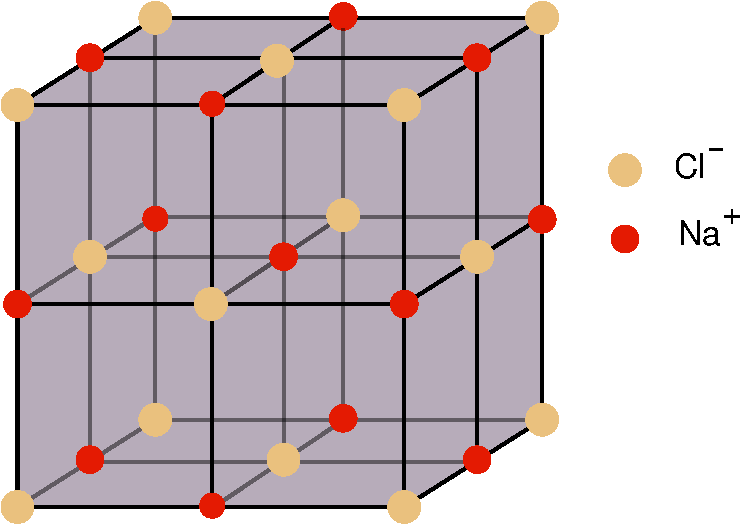
\includegraphics[width=0.35\textwidth]{nacl}
	\end{figure}
	\item Edge legth of unit cell of the NaCl type, a $=2(r_{Na^{+}}+r_{Cl^{-}})$\\
	Thus, the distance between  $Na^{+}$ and $Cl^{-}$ ions = $\frac{1}{2}a$
	\item On applying pressure, NaCl structure (6:6 coordination) changes to CsCl structure (8:8 coordination)
	\item The ionic radius of $Na^{+}$ ion (r = 95 pm) and the radius of $Cl^{-}$ ion (R = 181 pm) gives radius ratio r/R = 0.525 pm. This value suggest an octahedral arrangement of ions.
\end{itemize}
\begin{example}
	Alkali halides $\longrightarrow$ NaCl, KCl, LiCl, KBr, RbI, AgCl, AgBr, AgI, $NH_{4}Cl$, $NH_{4}Br$, $NH_{4}I$\\
	Oxides of alkaline earth metals $\longrightarrow$ MgO, CaO, TiO, FeO, NiO
\end{example}

\subsection{Structure of CsCl}
\begin{itemize}
	\item The space lattice is simple cubic
	\item The $Cl^{-}$ ions are present at the corners of the cubic unit cell and the $Cs^{+}$ ions are at the body centre of the unit cell\\
	i.e., one $Cs^{+}$ ion at (0 0 0) and one $Cl^{-}$ at $(\frac{1}{2}\ \frac{1}{2}\ \frac{1}{2})$
	\item The coordination number is 8. Thus it is an 8:8 coordination crystal.
	\begin{figure}[h]
		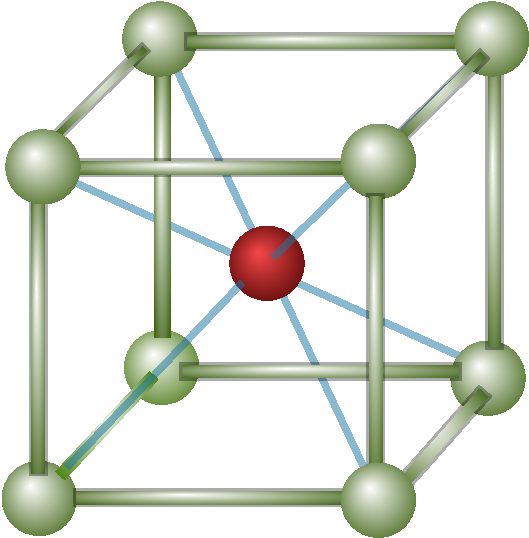
\includegraphics[width=0.28\textwidth]{cscl}
	\end{figure}
	\item At high temperature, CsCl structure changes to NaCl structure
	\item The ionic radii of $Cs^{+}$ and $Cl^{-}$ ions are 169 pm and 181 pm respectively. This gives the radius ratio as 0.93\\
	This value of radius ratio corresponds to BCC type of unit cell.
	\item The unit cell has contribution of one $Cs^{+}$ ion and one $Cl^{-}$ ion per unit cell.
	\item Relation between radius of cation, anion and edge length of the cube,\\
	$r_{Cs^{+}}	+r_{Cl^{-}} = \frac{a\sqrt{3}}{2}$
\end{itemize}
\begin{example}
	Examples: CsCl, CsBr, CsI, RbCl, LiHg
\end{example}

\subsection{Structure of ZnS}
\begin{itemize}
	\item Zinc sulphide exists in two forms: ZnS blende and ZnS Wurtzite
	\item\textbf{ Zinc blende} structure is almost identical to the diamond structure except that the two interpenetrating  FCC sub-lattices are of different atoms and displaced from each other by one- quarter of the body diagonal.
	\item The cubic ZnS structure results when Zn- atoms are placed on one FCC lattice and S- atoms on the other FCC lattice.\\
	\begin{figure}[h]
		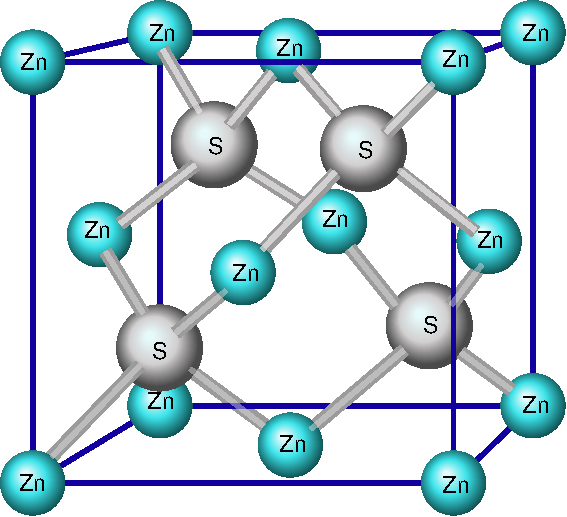
\includegraphics[width=0.35\textwidth]{zns}
	\end{figure}
	\item Each sulphide ion is surrounded by four $Zn^{2+}$ ions and each zinc ion is surrounded by four $S^{2-}$ ions. Therefore ZnS has 4:4 coordination.
	\item The ionic radii of $Zn^{2+}$ and $S^{2-}$ are 74pm and 184 pm respectively.\\
	$\therefore \text{Radius ratio}, \frac{r}{R}= 0.40$, which suggests the tetrahedral arrangement of ions in the crystal lattice.
	\item In a unit cell of ZnS, there will be four Zn- atoms and four S- atoms
	\begin{example}
		ZnS, CuCl, InSb, CdS, AgI, BeS
	\end{example}
	\item In\textbf{ Wurtzite structure} of ZnS, the sulphide ions are arranged in a \textit{hcp arrangement.}
	\begin{figure}[h]
		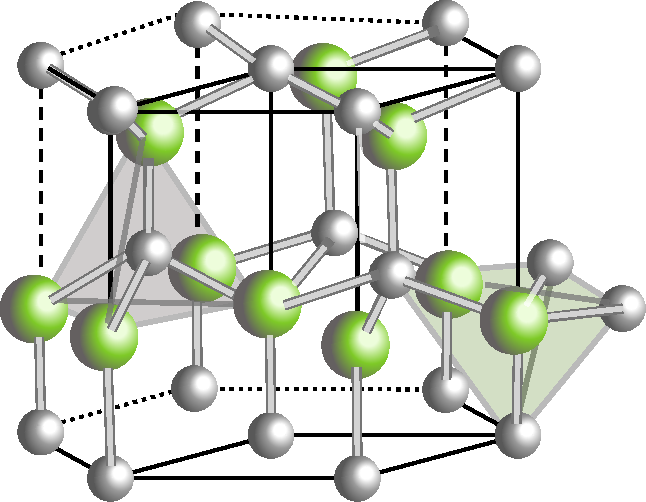
\includegraphics[width=0.35\textwidth]{wurtzite}
	\end{figure}
	\item The $Zn^{2+}$ ions occupy half of the tetrahedral sites.
	\item There are two tetrahedral sites for each $s^{2-}$ ion in the lattice. Since only half of them are occupied by $Zn^{2+}$ ions, the stoichiometry of the compound is 1:1
	\item  In wurtzite structure also ZnS has 4:4 coordination.
\end{itemize}
\begin{example}
	AgI, ZnO, $NH_{4}F$ and AlN
\end{example}
\subsection{Diamond Cubic Sturcture}
\begin{itemize}
	\item The diamond lattice can be considered to be formed by interpenetrating two fcc lattices along the body diagonal by $(\frac{1}{4})^{th}$ cube edge.
	\item One sublattice has its origin at the point (0, 0, 0) and the other at a point $(\frac{a}{4},\ \frac{a}{4}, \ \frac{a}{4})$
	\begin{figure}[h]
		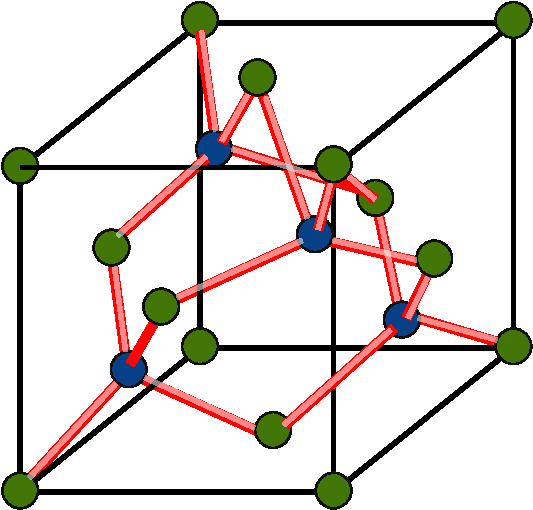
\includegraphics[width=0.30\textwidth]{diamond}	
	\end{figure}
	\item The point 0 and $\frac{1}{2}$ are on the fcc lattice, those at $\frac{1}{4} \ \text{and}\  \frac{3}{4}$ are on a similar lattice displaced among the body diagonal by $\frac{1}{4}$ of the cube edge.
	\item Each carbon atom has four nearest neighbours at distance, $\frac{\sqrt{3}a}{4}$
	\item There are 12 second nearest neighbours at distance $\frac{a}{\sqrt{2}}$
	\item Number of atoms per unit cell = 8
	\item Atomic packing fraction = $34 \%$
\end{itemize}
\begin{example}
	Carbon, Silicon, Germanium
\end{example}
\subsection{Structure of Graphite}
\begin{itemize}
	\item Graphite is a form of carbon and crystalises in simple hexagonal structure. It contains 4 atoms per primitive unit cell
	\item Number of nearest neighbour = 3
	\item One C- atom can make covalent bond with 3 nearby atoms.\\
	C- atoms of one layer can not bond with C- atom of second layer. That's why graphite sheets slides on each other. Therefore graphite is soft because layer do not have bonding
	\item Since, semiconductors are not conducting at T= 0K and metals are conducting at T= 0K, graphite is a semi-metal.
\end{itemize}	



\section{Crystal Defects}
Crystal defects are broadly classified into two types- \textbf{stoichiometric defects} and \textbf{non – stoichiometric defects. }
\subsection{Stoichimetric Defects}
\begin{itemize}
	\item Arises if the ratio between the cations and anions in the crystal remain same and the overall formula of ionic compound do not change.\\
	\textbf{1. Schottky Defect}
	
	\item In an ionic crystal of the type $A^{+}B^{-}$, equal number of cations and anions are missing from their lattice sites so that the electrical neutrality is maintained.
	\item The Schottky defet contains one pair of holes due to missing of one cation and one anion.\\
	\begin{minipage}{0.95\textwidth}
		\centering
		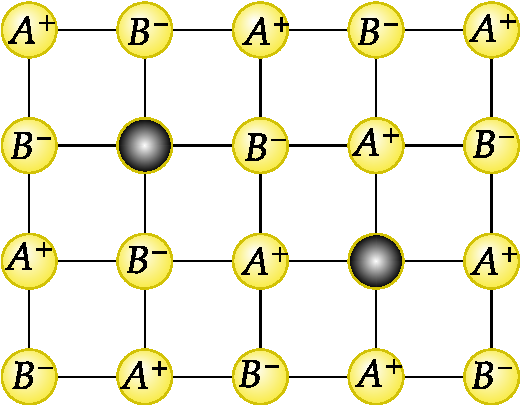
\includegraphics[width=0.35\textwidth]{schotky-crop}
	\end{minipage}
	\item This defect is shown by ionic compounds having high coordination number and Small difference in the size of cations and anions.
	\item As the number of ions decreases, the mass decreases whereas volume remains the same. Hence the density of the solid decreases.
	\item Example: NaCl, KCl, KBr, CsCl\\
	\textbf{2. Frenkel Defect}
	\item The cation is missing from the lattice site and it occupies the interstitial site.
	\item Electrical neutrality as well as the stoichiometry of the compound are maintained. \\
	\begin{minipage}{0.95\textwidth}
		\centering
		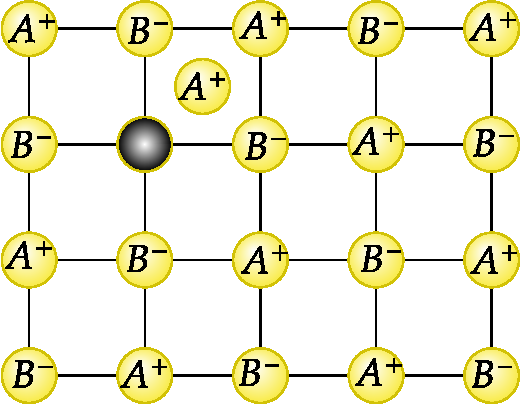
\includegraphics[width=0.35\textwidth]{frenkel-crop}
	\end{minipage}
\item This type of defect is present in compounds which have low coordination number and larger difference in the size of cations and anions
	\item Since no ions are missing from the crystal as a whole, therefore density of the solid remains unchanged. 
	\item Due to presence of holes, the stability (or the lattice energy) of the crystal decreases
	\item Example: Silver halides\\
	There are some ionic solids which show both Schottky and Frenkel defects (e.g. AgBr)
\end{itemize}
\begin{note}
	Crystalline solids having the above defects conduct electricity by \textbf{ionic mechanism}. Under the influence of an electrical field, an ion moves from its lattice site to an adjacent \textit{hole} (i.e., vacancy in the lattice), a new hole is created. Thus the hole moves in a direction opposite to that of the ion.
\end{note}
\textbf{Thermodynamics of Frenkel and Schottky Defect}\\
Although energy is used up in the formation of these defects, there is an accompanying increase in entropy, resulting in decrease of free energy. \\
For the Frenkel defect, we have the equilibrium, \\
\begin{alignat*}{3}
&\text{Ions occupying eq.lattice positions }&&+ \quad && \text{vacant interstitial positions}\\
&\left. \right. && \uparrow \downarrow && \left. \right. \\
&\text{Ions occupying interstitial positions} &&+ \quad && \text{vacant lattice positions}
\end{alignat*}
Similarly for Schottky defect, we have\\
\begin{alignat*}{3}
&\text{Cation and anion occupying normal lattice positions}&&+ \quad && \text{two hypothetical sites on the crystal surface}\\
&\left. \right. && \uparrow \downarrow && \left. \right. \\
&\text{Cation and anion lattice vacancies} &&+ \quad && \text{ion- pair adsorbed on the surface}
\end{alignat*}
\subsection{Non-stoichimetric defects}
\begin{itemize}
	\item Non- stoichiometric compounds are those in which the ratio of positive and negative ions in the compounds differ from that indicated by their ideal chemical formula.
	\item Example: $Fe_{0.95}O, Cu_{1.97}S$ etc.
	\item These defects arises due to excess of metal or non- metal atoms
\end{itemize}
\begin{enumerate}
	\item \textbf{Metal excess defect}
	\begin{itemize}
		\item Arises due to \textbf{\textit{missing of a negative ion}} from lattice site and position taken by an electron.
		\item This defect is simialr to Schottky defect and also found in crystals showing Schottky defect.\\
		\begin{minipage}{0.95\textwidth}
			\centering
			\includegraphics[width=0.35\textwidth]{me1}
		\end{minipage}
		\begin{example}
			When sodium vapours passed over NaCl crystal a yellow non- stoichiometric form of NaCl is obtained. Vacant lattice site occupied by electrons called \textbf{F- Centre} (Farbe colour), which is responsible for colour of crystal.
		\end{example}
		\item \textbf{An extra metal occupy interstitial site} and to maintain electrical neutrality, electrons occupy another interstitial site.\\
		\begin{minipage}{0.95\textwidth}
			\centering
			\includegraphics[width=0.35\textwidth]{me2}
		\end{minipage}
		\item This type of defect is very close to Frenkel defect.
		\begin{example}
			When ZnO is heated, it turns yellow as it's loses some oxygen. The $Zn^{2+}$ ion move to an interstitial site.
		\end{example}
		\item In this defect there is no hole in the crytal
		\item Crystals with metal excess defect contain free electrons and if these migrate, they conduct an electric currrent 
		\item As amount of current carried is very small, they behave like semiconductors (n- type semiconductor)
	\end{itemize}
	\item \textbf{Metal deficiency defect}
	\begin{itemize}
		\item \textbf{A positive ion may be absent} from a lattice site causing metal deficiency. 
		\item Electrical neutrality is then maintained by an adjacent metal ion having more charges. 
		\begin{example}
			FeO, FeS, NiO
		\end{example}
		\begin{minipage}{0.95\textwidth}
			\centering
			\includegraphics[width=0.45\textwidth]{md}
		\end{minipage}
		  \item Another possibility for metal deficiency is by \textbf{an extra negative ion} occupying an interstitial position.
		\item   The overall electrical neutrality is maintained here again by an adjacent metal ion with an extra charge. 
		\item Example: Examples of crystals with this type of defect are very rare.
		\item Crystal with metal deficiency defect behaves like p- type semiconductors
	\end{itemize}
\end{enumerate}
\newpage
\begin{abox}
	Magnetic Properties of Materials
\end{abox}	

\section{Magnetization}
\begin{wrapfigure}{r}{0.3\textwidth}
	\begin{center}
		\includegraphics[width=0.28\textwidth]{magnetic moment}
	\end{center}
	\caption{magnetic dipole moment}
\end{wrapfigure}
In a substance we have internal currents within a material because there are moving charges in atoms and molecules which can create their own magnetic field. Any current loop has a magnetic field and thus has a magnetic dipole moment.There are two types effects here, the first is due to the orbital motion of the electrons and the second is due to the intrinsic spin magnetic moment of the electrons. The second effect is purely quantum mechanical in origin . The magnetic moment could be intrinsic to an atom or molecule or it could be induced by an externally applied magnetic field. \par
Ordinarily, the current loops inside an object cancel each other out because of the random orientation of the atoms. But when a magnetic field is applied, a net alignment of these magnetic dipoles occurs, and the medium becomes magnetically polarized, or magnetized.
\\
Let ${m_{i}}$ be the magnetic moment of the $\mathrm{i}$ -th atom inside a matter. We define magnetization as the net magnetic moment per unit volume
$$
\vec{M}=\lim _{\Delta V \rightarrow 0} \frac{\sum_{i} {m_{i}}}{\Delta V}
$$
The magnetization is related to the appplied magnetic field strength by the realation,
\begin{equation}
M=\chi H
\end{equation}
Where $\chi$ is the \textbf{magnetic susceptibility} of the material and it is dimensionless.
\section{Magnetic Permeability}
If an unmagnetized bar of a magnetic material is placed in a uniform magnetic field as shown in Figure.\ref{Magnetic m1}  It has been observed that the bar gets magnetized by induction and gets a polarity. After magnetization, the mag. netic lines in the bar emanate from $\mathrm{N}$ pole, pass through the outer region and then re-enter the S-pole as in Figure.\ref{Magnetic m2}. These lines form a closed loop within the magnet by passing from $\mathrm{S}$-pole to $\mathrm{N}$-pole. It will be interesting to know, that the lines of the magnetized bar oppose the lines of the original field outside the magnet and favour inside the magnet.\\
\begin{center}

	\begin{figure}[H]
	\begin{minipage}{0.45\textwidth}
		\includegraphics[height=3cm,width=4cm]{Magnetic Permeability 1}
\end{minipage}\hfill
\begin{minipage}{0.45\textwidth}
		\includegraphics[height=3cm,width=4cm]{Magnetic Permeability 2}
\end{minipage}
\caption{}
\label{}
\end{figure}
\end{center}
The resultant field is shown in Fig. 9.1(b). As a result of this, the magnetic field strength (H) is increased inside the bar and decreased outside it. Similarly, the magnetic flux density (B) becomes high inside the bar and low outside. Thus we find that flux density (B) is directly proportional to the magnetic field strength (H). Mathematically
i.e.,

\begin{align*}
\mathbf{B} \propto \mathbf{H} \\
\mathbf{B}=\mu \mathbf{H}
\end{align*}

\subsection{Magnetic Materials}
Some materials are magnetic even without the application of any-magnetic field and become more magnetic when a weak magnetic field is applied to them. Many other materials lose their initially strong magnetism when heated above a certain critical temperature and become comparatively weakly magnetised.
Some materials show a magnetic response in a direction opposite to that of any externally applied field.\\ Based on the magnetic response, materials can be classified into the following three major groups:  Diamagnetism,  Paramagnetism,  and Ferromagnetism.
\begin{enumerate}
	\item \textbf{Diamagnetic:}
	Atom has no net magnetic moment, but a field induces a small moment opposite to the field. Susceptibility is negative $\left(\mu_{\mathrm{r}}<1\right)$
    \item \textbf{Paramagnet:} Atoms have a net moment but the spin directions are randomly arranged. An applied field can give weak alignment, hence a small susceptibility that varies with $1 / \mathrm{T}$. $\left(\mu_{\mathrm{r}}>1\right)$
	\item \textbf{Ferromagnet:} Have spontaneous magnetization, a large permeability which depends on the history of the sample, and nonlinear, hysteretic behavior. Depending on the effect of magnetisation Ferromagnetic substance are again classified in to two
	\begin{enumerate}
		\item Anti ferromagnetic
		\item Ferrimaganetic
	\end{enumerate}
\end{enumerate}

\paragraph{Diamagnetism}
\begin{figure}[H]
	\centering
	\includegraphics[height=4cm,width=12cm]{diagram-20211112(3)-crop}
	\caption{Flux density in(a) a diamagnetic (b)paramagnetic sample}
	\label{}
\end{figure}
Diamagnetism, a very weak fundamental property of all matter, arises due to the non-cooperative behavior of orbiting electrons when exposed to an externally applied magnetic field. 
\begin{itemize}
	\item  Very weak; exists only in presence of an external field, non-permanent.
	\item  Applied external field acts on atoms of a material, slightly unbalancing their orbiting electrons, and creates small magnetic dipoles within atoms which oppose the applied field. This action produces a negative magnetic effect known as diamagnetism.
	\item  The induced magnetic moment is small, and the magnetization $(M)$ direction is opposite to the direction of applied field $(H)$.
	\item  Thus the relative permeability is less than unity i.e. magnetic susceptibility $(\chi_{m})$ is negative, and is in order of $-10^{-5}$.
	\item  Materials such as $\mathrm{Cu}, \mathrm{Ag}, \mathrm{Si}$,  and alumina are diamagnetic at room temperature.
\end{itemize}
\begin{note}
	\begin{itemize}
		\item Susceptibility of diamagnetic material is is negative and independant of temperature.
		\item The susceptibility of diamagnetic substances is directly proportional to the atomic number. The bigger would be the value of the susceptibility if the atom is bigger.
		\item  Almost all materials exhibit diamagnetism though it is masked by the other magnetic effects. 
		\item Diamagnetism is attributed to the influence of the magnetic field on the \textbf{orbital momentum} of the electrons. Although s-electrons have a zero angular momentum in the absence of a magnetic field, yet they acquire a small amount of orbital momentum upon the application of field. This explains why all the electrons in an atom contribute to diamagnetism.
	\end{itemize}
\end{note}
\paragraph{Paramagnetism}
Materials which exhibit a small positive magnetic susceptibility in the presence of a magnetic field are called para-magnetic, and the effect is termed as para-magnetism.
This class of the materials has a net magnetic moment due to the existence of unpaired electrons in partially filled orbitals. However, the individual magnetic moments do not interact magnetically and hence the magnetization is zero when there is no external applied field or when the externally applied field is removed.
\begin{itemize}
	\item  Slightly stronger than Diamagnetism. When an external field is applied dipoles line-up with the field, resulting in a positive magnetization. However, the dipoles do not interact.
	
	\item In the absence of an external field, the orientations of atomic magnetic moments are random leading to no net magnetization.
	\item  When an external field is applied dipoles line-up with the field, resulting in a positive magnetization.
	- However, because the dipoles do not interact, extremely large magnetic fields are required to align all of the dipoles.
	\item  In addition, the effect is lost as soon as the magnetic field is removed.
	\item  Since thermal agitation randomizes the directions of the magnetic dipoles, an increase in temperature decreases the paramagnetic effect.
	\item Magnetic susceptibility $(\chi_{m})$  of these materials is slightly positive, and lies in the range $+10^{-5}$ to $+10^{-2}$
	\item  Para-magnetism is produced in many materials like aluminium, calcium, titanium, alloys of copper.
\end{itemize}
\begin{figure}[H]
	\centering
	\includegraphics[height=4cm,width=8cm]{diagram-20211112(2)-crop}
	\caption{Variation of $\chi$ Vs Temperature of paramagnetic material.}
	\label{}
\end{figure}


\subsection{Ferromagnetism} 
Certain materials possess permanent magnetic moments even in the absence of an external field, These are called Ferromagnetic materials.
The atomic moments in these materials exhibit very strong interactions. These interactions are produced by electronic exchange forces and result in either a parallel or an antiparallel alignment of atomic moments 
\begin{itemize}
	\item  Both dia- and para- magnetic materials are considered as non-magnetic because they exhibit magnetization only in presence of an external field.
	
	\item  The permennat dipoles can easily line-up with the imposed magnetic field due to the exchange interaction or mutual reinforcement of the dipoles. These are chrematistics of ferromagnetism.
	\item  Materials with ferro-magnetism (Examples: Fe, Co, Ni, Gd) possess magnetic susceptibilities approaching $10^{6}$.
	\item  Above a specific temperature called Curie temperature, ferro-magnetic materials behave as para-magnetic materials and their susceptibility is given by the Curie-Weiss law, defined as
	$$
	\chi_{m}=\frac{C}{T-T_{c}}
	$$
	Where $C$ - material constant, $T-$ temperature, $T_{c}-$ Curie temperature.
	\item  Ferro Magnets are very strong; dipoles line-up permanently upon application of external field. Has two sub-classes:-
	\begin{itemize}
		\item Anti-ferro-magnetism.
		\item  Ferri-magnetism
	\end{itemize}
	
\end{itemize}
\begin{figure}[H]
	\centering
	\includegraphics[height=5cm,width=5cm]{diagram-20211112(4)-crop}
	\caption{}
	\label{}
\end{figure}

 \subsubsection{Antiferromagnetism}
 These are other effects that lead to a cancelling (antiferromagnetism)  of the magnetism of different atoms. In antiferromagnetic materials the resultant magnetization vanishes in the absence of a field. The atomic dipoles are arranged antiparallel to one another so that the net moment is zero. Above the \textbf{Neel temperature} $\mathrm{T}_{\mathrm{N}}$, the dipoles are randomly oriented as in a paramagnet. $\mathrm{NiO}, \mathrm{MnS}, \mathrm{MnO}$ are some examples.
 \begin{figure}[H]
 	\centering
 	\includegraphics[height=4cm,width=6cm]{diagram-20211112(1)-crop}
 	\caption{}
 	\label{}
 \end{figure}
\subsubsection{Ferrimagnetism}
  The atomic dipoles in ferrimagnetic materials are antiparallel to one another but the moments in one direction have a longer magnitude so that the net magnetization is non zero. Some examples of this category of materials are $\mathrm{Fe}_{3} \mathrm{O}_{4}$, yttrium iron garnet $\left(\mathrm{Y}_{3} \mathrm{Fe}_{5} \mathrm{O}_{12}\right)$ and nickel ferrite $\left(\mathrm{NiFe}_{2} \mathrm{O}_{3}\right) .$ Ferrimagnetic materials become paramagnetic above the curie temperature $\left(T_{c}\right)$.
 
  \subsection{Fermi Energy}
  The number of electrons having fermi energy at temperature $T=0K$ is \\
  $$N=\left( \frac{\pi}{3}\right) \left[ \frac{8m}{h^2}\right]^{\frac{3}{2}}VE_F^{\frac{3}{2}}$$
  Therefore the number of electrons per unit volume (called density of electrons) is
  $$
  n=\frac{N}{V}=\frac{\pi}{3}\left[\frac{8 m}{h^{2}}\right]^{3 / 2} E_{F}^{3 / 2}
  $$
  $$
  \begin{aligned}
  	E_{F}^{3 / 2} &=\left(\frac{3 n}{\pi}\right)\left[\frac{h^{2}}{8 m}\right]^{3 / 2} \\
  	E_{F} &=\left(\frac{h^{2}}{8 m}\right)\left[\frac{3 n}{\pi}\right]^{2 / 3} \\
  	E_{F} &=\left(\frac{h^{2}}{2 m}\right)\left[\frac{3 n}{8 \pi}\right]^{2 / 3}=0.58 \times 10^{-37} n^{2/3} \text { joule } \\
  	E_{F}=3.65 \times 10^{-19} n^{2 / 3}(\text { in electron volt }) &
  \end{aligned}
  $$
  This expression of Fermi energy is a very useful quandity.\\
  \textbf{Fermi energy at T$\neq$ 0K}
  $$E_f=E_F\left[ 1-\frac{\pi^2}{12}\left( \frac{k_BT}{E_F}\right) ^2\right] $$
  \textbf{Fermi velocity}
  $$\frac{1}{2}mV_F^2=E_F$$
  $$V_F^2=\frac{2E_F}{m}$$
  \textbf{Fermi temperature}
  $$k_BT_F=E_F$$
  $$T_F=\frac{E_F}{k_F}$$
  \begin{exercise}
  Fermi energy of copper is $7 \mathrm{eV}$ at room temperature. What is the total number of free electrons/unit volume at the same temperature? 
  \end{exercise}
\begin{answer}
$$	E_{F}=3.65 \times 10^{-19} n^{2 / 3}(\text { in electron volt }) $$
$E_f=7eV$\\
$$n^{\frac{2}{3}}=\frac{7\times 10^{19}}{3.65}$$
$$n=8.2\times 10^{28}$$
\end{answer}
\begin{exercise}
	 The Fermi energy of silver is  $5.5 \mathrm{eV}$ and the relaxation time of electrons is $3.97 \times 10^{-14} \mathrm{~s}$  Calculate the Fermi velocity and the mean free path for the electrons in silver.
\end{exercise}
\begin{answer}
	We know that $\frac{1}{2} m v_{F}^{2}=E_{F}$
	or $\quad V_{\mathrm{F}}=\sqrt{\frac{2 E_{F}}{m}}=\sqrt{\frac{2 \times 5.5 \times 1.602 \times 10^{-19}}{9.11 \times 10^{-31}}}$
	$$
	1.39 \times 10^{6} \mathrm{~m} / \mathrm{s}
	$$
	The mean free path, $\lambda=V_{F} \tau$
	$$
	\begin{aligned}
	&=1.39 \times 10^{6} \times 3.97 \times 10^{-14} \\
	&=5.52 \times 10^{-8} \mathrm{~m}
	\end{aligned}
	$$
\end{answer}

\newpage
\begin{abox}
	Practice Problems
\end{abox}
\begin{enumerate}
	\begin{minipage}{\textwidth}
		\item The inter-planar distance between (100) set of planes in a face cantered cubic unit cell is $170 \mathrm{pm}$. The distance between two $(200)$ set of planes is
	\end{minipage}
	\begin{answer}
		For an FCC lattice,
		$$
		\begin{aligned}
		d_{h k l} &=\frac{a}{\sqrt{h^{2}+k^{2}+l^{2}}} \\
		d_{100} &=\frac{a}{\sqrt{h^{2}+k^{2}+l^{2}}}=170 \mathrm{pm} \\
		\therefore a &=170 \mathrm{pm}
		\end{aligned}
		$$
		Now, $d_{200}=\frac{170}{\sqrt{2^{2}+0^{2}+0^{2}}}$
		$$
		\begin{aligned}
		&=\frac{170}{2} \\
		&=85 \mathrm{pm}
		\end{aligned}
		$$	
	\end{answer}
	\begin{minipage}{\textwidth}
		\item Copper crystallises in a face-centred cubic lattice with a unit cell length of $361 \mathrm{pm}$. What is the radius of copper atom in $\mathrm{pm}$ ? 
	\end{minipage}
	\begin{answer}
		For an FCC lattice,
		$$
		\begin{aligned}
		r &=\frac{\sqrt{2}}{4} a \\
		&=\frac{\sqrt{2}}{4} \times 361 \approx 127 \mathrm{pm}
		\end{aligned}
		$$	
	\end{answer}
	\begin{minipage}{\textwidth}
		\item  The angle between the Miller planes (110) and (100) in a simple cubic lattice is
	\end{minipage}
	\begin{answer}
		$$\begin{aligned}
		\cos \theta &=\frac{h_{1} h_{2}+k_{1} k_{2}+l_{1} l_{2}}{\sqrt{h_{1}^{2}+k_{1}^{2}+l_{1}^{2}} \sqrt{h_{2}^{2}+k_{2}^{2}+l_{2}^{2}}} \\
		&=\frac{(1 \times 1)+(1 \times 0)+(0 \times 0)}{\sqrt{1^{2}+1^{2}+0^{2}} \sqrt{1^{2}+0^{2}+0^{2}}} \\
		\cos \theta &=\frac{1}{\sqrt{2}} \\
		\theta &=45^{0}
		\end{aligned}$$	
	\end{answer}
	\begin{minipage}{\textwidth}
		\item The correct relationship among the following, for a tetragonal $\left(a=b \neq c ; \alpha=\beta=\gamma=90^{0}\right)$ crystal system is
	\end{minipage}
	\begin{answer}
		$$
		\begin{aligned}
		\frac{1}{d^{2}} &=\frac{h^{2}}{a^{2}}+\frac{k^{2}}{b^{2}}+\frac{l^{2}}{c 2} \\
		\because 2 d \sin \theta &=\lambda \\
		4 d^{2} \sin ^{2} \theta &=\lambda^{2}
		\end{aligned}
		$$
		I $\mathrm{t}$ is given that $\mathrm{a}=\mathrm{b}$. Therefore,
		$$
		\begin{aligned}
		\sin ^{2} \theta &=\frac{\lambda^{2}}{4}\left(\frac{h^{2}}{a^{2}}+\frac{k^{2}}{a^{2}}+\frac{l^{2}}{c 2}\right) \\
		\sin ^{2} \theta &=\frac{\lambda^{2}}{4}\left(\frac{c^{2}\left(h^{2}+k^{2}\right)+a^{2} l^{2}}{a^{2} c^{2}}\right) \\
		\sin ^{2} \theta &=\frac{\lambda^{2}}{4 a^{2} c^{2}}\left[c^{2}\left(h^{2}+k^{2}\right)+a^{2} l^{2}\right]
		\end{aligned}
		$$	
	\end{answer}
	\begin{minipage}{\textwidth}
		\item Metallic silver crystallizes in face- centred-cubic lattice structure with a unit cell of length $40 \mathrm{~nm}$. The first order diffraction angle of $\mathrm{X}$-ray beam from $\left(\begin{array}{lll}2 & 1 & 0\end{array}\right)$ plane of silver is $30^{\circ} .$ The wavelength of $X$ - ray used is close to
	\end{minipage}
	\begin{answer}
		According to Bragg's equation,
		$$
		n \lambda=2 d \sin \theta
		$$
		It is given that,
		$$
		\mathrm{a}=40 \mathrm{~nm} ;(\mathrm{h}, \mathrm{k}, \mathrm{l})=(210) ; \theta=30^{\circ}
		$$
		$$
		\begin{aligned}
		\lambda &=2 \times\left(\frac{a}{\sqrt{h^{2}+k^{2}+l^{2}}}\right) \times \sin (\theta) \\
		\lambda &=2 \times\left(\frac{40 \mathrm{~nm}}{\sqrt{2^{2}+1^{2}+0^{2}}}\right) \times \sin \left(30^{0}\right) \\
		& \approx 18 \mathrm{~nm}
		\end{aligned}
		$$	
	\end{answer}
	\begin{minipage}{\textwidth}
		\item Consider an orthorhombic cell of dimensions $\mathrm{a}=450 \mathrm{pm}, \mathrm{b}=650 \mathrm{pm}, \mathrm{c}=400 \mathrm{pm} .$ The perpendicular distance between the $\left(\begin{array}{lll}1 & 1 & 0\end{array}\right)$ planes is
	\end{minipage}
	\begin{answer}
		$$
		\begin{aligned}
		\frac{1}{d_{h k l}^{2}} &=\frac{h^{2}}{a^{2}}+\frac{k^{2}}{b^{2}}+\frac{l^{2}}{c^{2}} \\
		&=\frac{1^{2}}{450^{2}}+\frac{1^{2}}{650^{2}}+\frac{0^{2}}{400^{2}} \\
		&=\frac{1^{2}}{450^{2}}+\frac{1^{2}}{650^{2}} \\
		&=\frac{(650)^{2}+(450)^{2}}{(450)^{2}(650)^{2}} \\
		&=\frac{422500+202500}{450 \times 450 \times 60 \times 650} \\
		d_{h k l}^{2} &=\frac{85556250000}{625000}=136890 \\
		d_{h k l} &=\sqrt{136890} \approx 370 \mathrm{pm}
		\end{aligned}
		$$	
	\end{answer}
	\begin{minipage}{\textwidth}
		\item Gold crystallizes in face- centred- cubic lattice. The atomic weight and density of gold are $196.97$ and $19.4 \mathrm{gcm}^{-3}$ respectively. The length of the unit cell is
	\end{minipage}
	\begin{answer}
		$$
		\begin{aligned}
		\rho &=\frac{Z M}{N a^{3}} \\
		a &=\left(\frac{Z M}{N \rho}\right)^{\frac{1}{3}} \\
		&=\left(\frac{4 \times 196.97}{6.023 \times 10^{23} \times 194} \mathrm{~cm}^{-3}\right)^{\frac{1}{3}} \\
		&=\left(6.7428 \times 10^{-23} \mathrm{~cm}^{3}\right)^{\frac{1}{3}}=\left(67.428 \times 10^{-24} \mathrm{~cm}^{3}\right)^{\frac{1}{3}} \\
		&=4.070 \times 10^{-8} \mathrm{~cm} \\
		&=4.070 A^{0}
		\end{aligned}
		$$	
	\end{answer}
	\begin{minipage}{\textwidth}
		\item For a simple cubic crystal, X- ray diffraction shows intense reflections for angle $\theta_{1}$ and $\theta_{2}$ which are assigned to $\left(\begin{array}{lll}1 & 0 & 1\end{array}\right)$ and $\left(\begin{array}{lll}1 & 1 & 1\end{array}\right)$ planes respectively. The ratio $\sin \theta_{1} / \sin \theta_{2}$ is
	\end{minipage}
	\begin{answer}
		$$
		\begin{aligned}
		2 d_{(101)} \sin \theta_{1} &=2 d_{(111)} \sin \theta_{2} \\
		\frac{\sin \theta_{1}}{\sin \theta_{2}} &=\frac{d_{(111)}}{d_{(101)}} \\
		d_{(111)} &=\frac{a}{\sqrt{1^{2}+1^{2}+1^{2}}}=\frac{a}{\sqrt{3}} \\
		d_{(101)} &=\frac{a}{\sqrt{1^{2}+0^{2}+1^{2}}}=\frac{a}{\sqrt{2}} \\
		\frac{\sin \theta_{1}}{\sin \theta_{2}} &=\frac{\frac{a}{\sqrt{3}}}{\frac{a}{\sqrt{2}}} \\
		&=\sqrt{\frac{2}{3}} \\
		&=0.816 \approx 0.82
		\end{aligned}
		$$	
	\end{answer}
	\begin{minipage}{\textwidth}
		\item The magnetic flux density within a bar of some material is $0.63$ Tesla at an $\mathrm{H}$ field of $5 \mathrm{X} 10^{5}$ A/m. Compute the following for this material:\\ (a) Magnetic permeability, \\(b) Magnetic susceptibility\\ (c) Type of magnetism that you suggest being displayed by the material with reasons.
	\end{minipage}
	\begin{answer}$\left. \right. $\\
		(a) Magnetic permeability, 
		\begin{align*}
		\mu&=\frac{B}{H}=\frac{0.63}{5 X 10^{5}}\\&=0.126 X 10^{-5} \mathrm{H} / \mathrm{m}
		\end{align*}
		(b) Magnetic susceptibility,
		\begin{align*}
		x&=\mu_{r}-1=\frac{\mu}{\mu_{0}}-1\\&=\frac{0.126 X 10^{-5}}{4 \pi X 10^{-7}}-1\\&=1.003185-1=0.003185
		\end{align*}
		(c) Type of magnetism: Paramagnetism since the magnetic suscptibility is positive and low in magnitude.
	\end{answer}
	\begin{minipage}{\textwidth}
		\item The density of silver is $10.5 \mathrm{~g} / \mathrm{cm}^{3}$  and its atomic weight is  $108$ If each atom contributes one electron for conduction, what is the fermi energy?
	\end{minipage}
	\begin{answer}
		Fermi Energy, $$E_{F}=\frac{h^{2}}{8 m}\left(\frac{3 N}{\pi v}\right)^{2 / 3}$$
		Here, N $$ \mathrm{V}=10.5 \times 6.02 \times 10^{23} / 108
		=5.85 \times 10^{28} \mathrm{~m}^{-3}$$
		Therefore, $$E_{F}=\frac{6.626 \times 6.626}{8 X 9.1} \times 10^{-19} \times \frac{3 \times 5.585}{\pi}^{2 / 3}$$  $$=8.816 \times 10^{-19} \mathrm{~J}$$
		$$=5.51 \mathrm{eV}$$.	
	\end{answer}
\end{enumerate}